\documentclass{article}
\usepackage{lmodern}
\usepackage[T1]{fontenc}
\usepackage{shapepar}
\usepackage{microtype}
\usepackage{lipsum}
\usepackage{pgfplots}
\pgfplotsset{compat=1.9}
\usepackage{tikz}
\usetikzlibrary{calc,fit,intersections,folding}
\usepackage{pstricks-add}
\usetikzlibrary{arrows.meta,angles,arrows,quotes,backgrounds}

\usepackage[a2paper, landscape, left = 1cm, right = 1cm, top=1cm, bottom = 1cm]{geometry}

\newcommand{\tubecolor}{blue}
\newcommand{\thickness}{0.5mm}
\newcommand{\n}{2.5mm}

\newcommand{\base}{
    \node[circle, fill] (s1) at (0,0) {};
    \node[circle, fill] (s2) at (4,0) {};
    \node[circle, fill] (l11) at (-1,-2) {};
    \node[circle, fill] (l12) at (1,-2) {};
    \node[circle, fill] (l21) at (3,-2) {};
    \node[circle, fill] (l22) at (5,-2) {};
    \draw[gray] (s1) -- (s2) (s1) -- (l11) (s1) -- (l12);
    \draw[gray] (s2) -- (l21) (s2) -- (l22);
}



\begin{document}
\thispagestyle{empty}
\begin{center}
    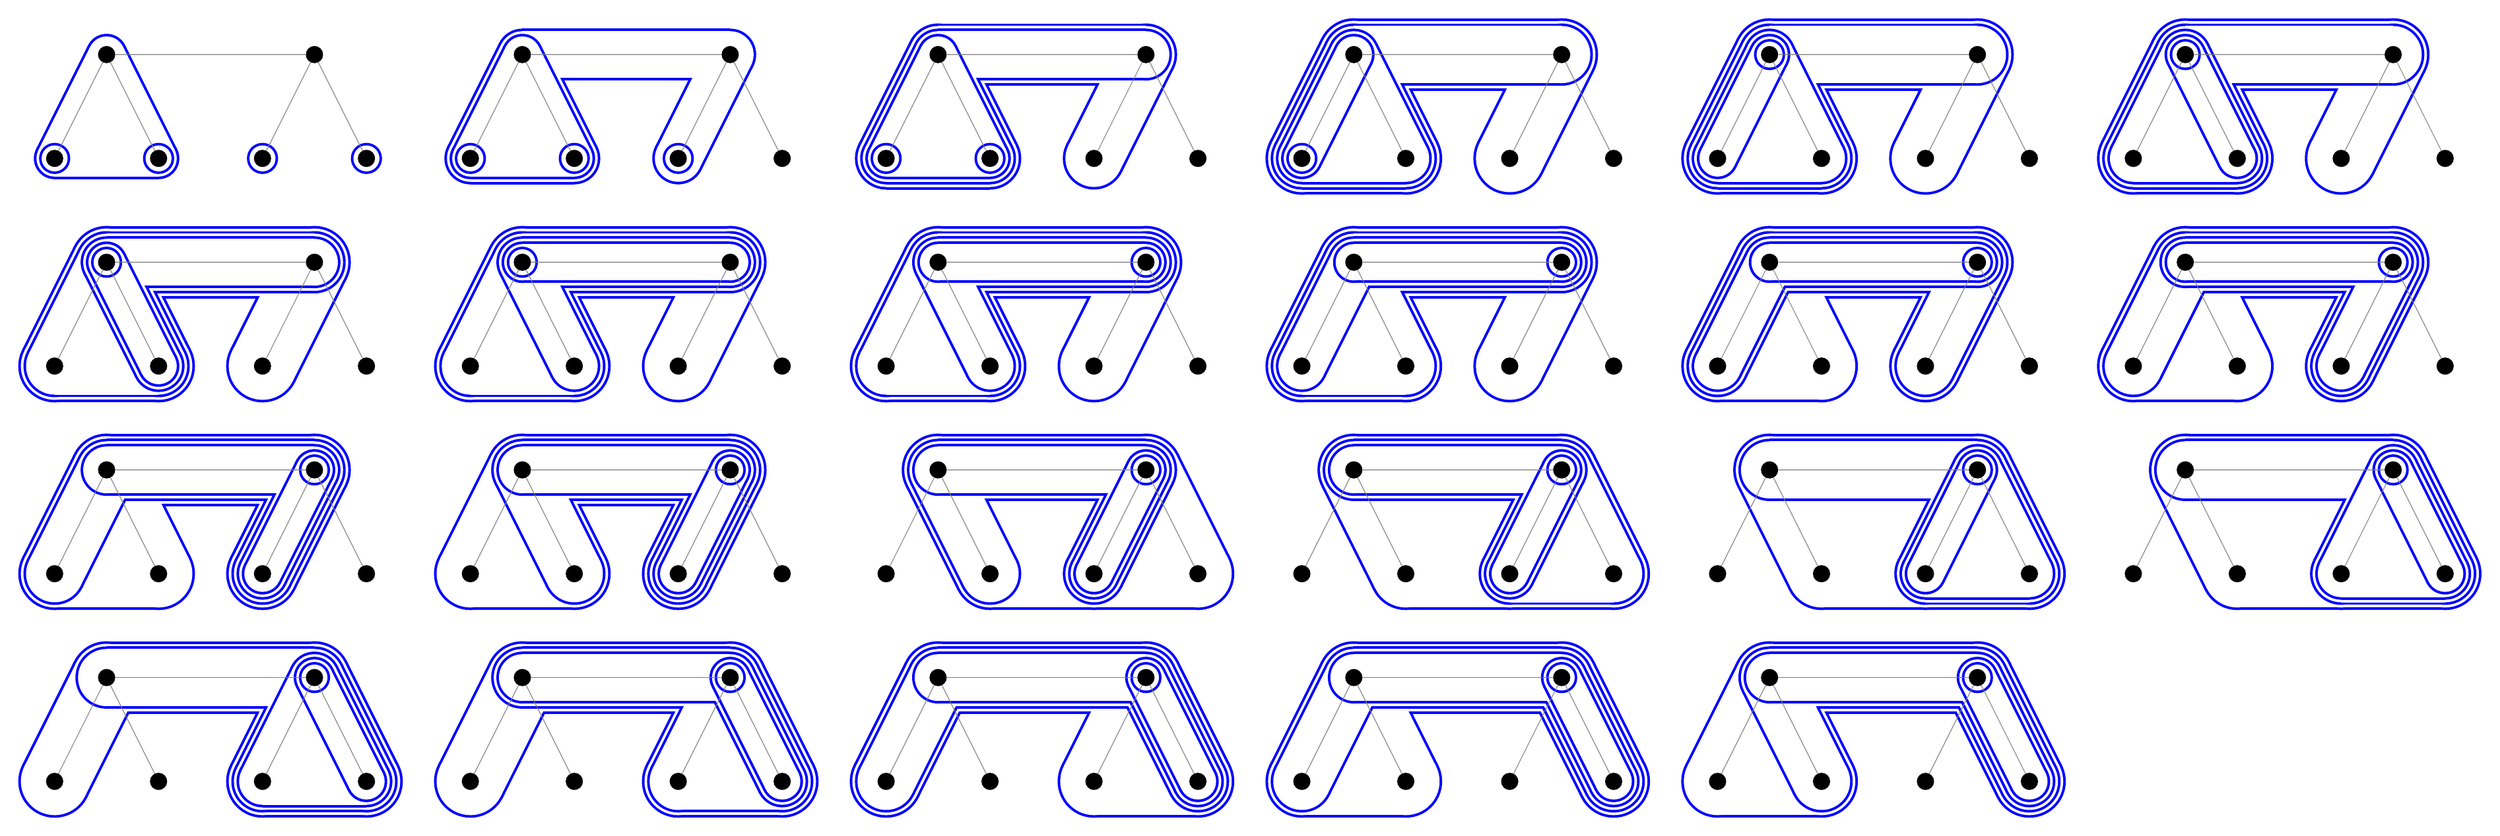
\begin{tikzpicture}

        \begin{scope}[xshift = 0cm, yshift = 0cm]
            \base
            \begin{scope}[on background layer]
                \fill[\tubecolor] (l22) circle (\n + 1*\thickness);
                
                \fill[white] (l22) circle (\n + 0*\thickness);
            \end{scope}
    
            \begin{scope}[on background layer]
                \fill[\tubecolor] (l21) circle (\n + 1*\thickness);
                
                \fill[white] (l21) circle (\n + 0*\thickness);
            \end{scope}
    
            \begin{scope}[on background layer]
                \fill[\tubecolor] (s1) circle (\n + 3*\thickness);
                \fill[\tubecolor] (l11) circle (\n + 3*\thickness);
                \fill[\tubecolor] (l12) circle (\n + 3*\thickness);
                \draw[\tubecolor] [line width = 2*(\n + 3*\thickness)] (s1.center) -- (l11.center);
                \draw[\tubecolor] [line width = 2*(\n + 3*\thickness)] (s1.center) -- (l12.center);
                \draw[\tubecolor] [line width = 2*(\n + 3*\thickness)] (l11.center) -- (l12.center);
                
                \fill[white] (s1) circle (\n + 2*\thickness);
                \fill[white] (l11) circle (\n + 2*\thickness);
                \fill[white] (l12) circle (\n + 2*\thickness);
                \draw[white] [line width = 2*(\n + 2*\thickness)] (s1.center) -- (l11.center);
                \draw[white] [line width = 2*(\n + 2*\thickness)] (s1.center) -- (l12.center);
                \draw[white] [line width = 2*(\n + 2*\thickness)] (l11.center) -- (l12.center);
                \fill[white] (s1.center) -- (l11.center) -- (l12.center) -- cycle;
            \end{scope}
    
            \begin{scope}[on background layer]
                \fill[\tubecolor] (l12) circle (\n + 1*\thickness);
                
                \fill[white] (l12) circle (\n + 0*\thickness);
            \end{scope}
            
            \begin{scope}[on background layer]
                \fill[\tubecolor] (l11) circle (\n + 1*\thickness);
                
                \fill[white] (l11) circle (\n + 0*\thickness);
            \end{scope}
        \end{scope}

        \begin{scope}[xshift = 8cm, yshift = 0cm]
            \base
            \begin{scope}[on background layer]
                \fill[\tubecolor] (s1) circle (\n + 5*\thickness);
                \fill[\tubecolor] (l11) circle (\n + 5*\thickness);
                \fill[\tubecolor] (l12) circle (\n + 5*\thickness);
                \fill[\tubecolor] (s2) circle (\n + 5*\thickness);
                \fill[\tubecolor] (l21) circle (\n + 5*\thickness);
                \draw[\tubecolor] [line width = 2*(\n + 5*\thickness)] (s1.center) -- (l11.center);
                \draw[\tubecolor] [line width = 2*(\n + 5*\thickness)] (s1.center) -- (l12.center);
                \draw[\tubecolor] [line width = 2*(\n + 5*\thickness)] (l11.center) -- (l12.center);
                \draw[\tubecolor] [line width = 2*(\n + 5*\thickness)] (s1.center) -- (s2.center);
                \draw[\tubecolor] [line width = 2*(\n + 5*\thickness)] (s2.center) -- (l21.center);
                
                \fill[white] (s1) circle (\n + 4*\thickness);
                \fill[white] (l11) circle (\n + 4*\thickness);
                \fill[white] (l12) circle (\n + 4*\thickness);
                \fill[white] (s2) circle (\n + 4*\thickness);
                \fill[white] (l21) circle (\n + 4*\thickness);
                \draw[white] [line width = 2*(\n + 4*\thickness)] (s1.center) -- (l11.center);
                \draw[white] [line width = 2*(\n + 4*\thickness)] (s1.center) -- (l12.center);
                \draw[white] [line width = 2*(\n + 4*\thickness)] (l11.center) -- (l12.center);
                \draw[white] [line width = 2*(\n + 4*\thickness)] (s1.center) -- (s2.center);
                \draw[white] [line width = 2*(\n + 4*\thickness)] (s2.center) -- (l21.center);
                \fill[white] (s1.center) -- (l11.center) -- (l12.center) -- cycle;
            \end{scope}
    
            \begin{scope}[on background layer]
                \fill[\tubecolor] (l21) circle (\n + 1*\thickness);
                
                \fill[white] (l21) circle (\n + 0*\thickness);
            \end{scope}
    
            \begin{scope}[on background layer]
                \fill[\tubecolor] (s1) circle (\n + 3*\thickness);
                \fill[\tubecolor] (l11) circle (\n + 3*\thickness);
                \fill[\tubecolor] (l12) circle (\n + 3*\thickness);
                \draw[\tubecolor] [line width = 2*(\n + 3*\thickness)] (s1.center) -- (l11.center);
                \draw[\tubecolor] [line width = 2*(\n + 3*\thickness)] (s1.center) -- (l12.center);
                \draw[\tubecolor] [line width = 2*(\n + 3*\thickness)] (l11.center) -- (l12.center);
                
                \fill[white] (s1) circle (\n + 2*\thickness);
                \fill[white] (l11) circle (\n + 2*\thickness);
                \fill[white] (l12) circle (\n + 2*\thickness);
                \draw[white] [line width = 2*(\n + 2*\thickness)] (s1.center) -- (l11.center);
                \draw[white] [line width = 2*(\n + 2*\thickness)] (s1.center) -- (l12.center);
                \draw[white] [line width = 2*(\n + 2*\thickness)] (l11.center) -- (l12.center);
                \fill[white] (s1.center) -- (l11.center) -- (l12.center) -- cycle;
            \end{scope}
    
            \begin{scope}[on background layer]
                \fill[\tubecolor] (l12) circle (\n + 1*\thickness);
                
                \fill[white] (l12) circle (\n + 0*\thickness);
            \end{scope}
            
            \begin{scope}[on background layer]
                \fill[\tubecolor] (l11) circle (\n + 1*\thickness);
                
                \fill[white] (l11) circle (\n + 0*\thickness);
            \end{scope}
        \end{scope}

        \begin{scope}[xshift = 16cm, yshift = 0cm]
            \base
            \begin{scope}[on background layer]
                \fill[\tubecolor] (s1) circle (\n + 7*\thickness);
                \fill[\tubecolor] (l11) circle (\n + 7*\thickness);
                \fill[\tubecolor] (l12) circle (\n + 7*\thickness);
                \fill[\tubecolor] (s2) circle (\n + 7*\thickness);
                \fill[\tubecolor] (l21) circle (\n + 7*\thickness);
                \draw[\tubecolor] [line width = 2*(\n + 7*\thickness)] (s1.center) -- (l11.center);
                \draw[\tubecolor] [line width = 2*(\n + 7*\thickness)] (s1.center) -- (l12.center);
                \draw[\tubecolor] [line width = 2*(\n + 7*\thickness)] (l11.center) -- (l12.center);
                \draw[\tubecolor] [line width = 2*(\n + 7*\thickness)] (s1.center) -- (s2.center);
                \draw[\tubecolor] [line width = 2*(\n + 7*\thickness)] (s2.center) -- (l21.center);
                
                \fill[white] (s1) circle (\n + 6*\thickness);
                \fill[white] (l11) circle (\n + 6*\thickness);
                \fill[white] (l12) circle (\n + 6*\thickness);
                \fill[white] (s2) circle (\n + 6*\thickness);
                \fill[white] (l21) circle (\n + 6*\thickness);
                \draw[white] [line width = 2*(\n + 6*\thickness)] (s1.center) -- (l11.center);
                \draw[white] [line width = 2*(\n + 6*\thickness)] (s1.center) -- (l12.center);
                \draw[white] [line width = 2*(\n + 6*\thickness)] (l11.center) -- (l12.center);
                \draw[white] [line width = 2*(\n + 6*\thickness)] (s1.center) -- (s2.center);
                \draw[white] [line width = 2*(\n + 6*\thickness)] (s2.center) -- (l21.center);
                \fill[white] (s1.center) -- (l11.center) -- (l12.center) -- cycle;
            \end{scope}
    
            \begin{scope}[on background layer]
                \fill[\tubecolor] (s1) circle (\n + 5*\thickness);
                \fill[\tubecolor] (l11) circle (\n + 5*\thickness);
                \fill[\tubecolor] (l12) circle (\n + 5*\thickness);
                \fill[\tubecolor] (s2) circle (\n + 5*\thickness);
                \draw[\tubecolor] [line width = 2*(\n + 5*\thickness)] (s1.center) -- (l11.center);
                \draw[\tubecolor] [line width = 2*(\n + 5*\thickness)] (s1.center) -- (l12.center);
                \draw[\tubecolor] [line width = 2*(\n + 5*\thickness)] (l11.center) -- (l12.center);
                \draw[\tubecolor] [line width = 2*(\n + 5*\thickness)] (s1.center) -- (s2.center);
                
                \fill[white] (s1) circle (\n + 4*\thickness);
                \fill[white] (l11) circle (\n + 4*\thickness);
                \fill[white] (l12) circle (\n + 4*\thickness);
                \fill[white] (s2) circle (\n + 4*\thickness);
                \draw[white] [line width = 2*(\n + 4*\thickness)] (s1.center) -- (l11.center);
                \draw[white] [line width = 2*(\n + 4*\thickness)] (s1.center) -- (l12.center);
                \draw[white] [line width = 2*(\n + 4*\thickness)] (l11.center) -- (l12.center);
                \draw[white] [line width = 2*(\n + 4*\thickness)] (s1.center) -- (s2.center);
                \fill[white] (s1.center) -- (l11.center) -- (l12.center) -- cycle;
            \end{scope}
    
            \begin{scope}[on background layer]
                \fill[\tubecolor] (s1) circle (\n + 3*\thickness);
                \fill[\tubecolor] (l11) circle (\n + 3*\thickness);
                \fill[\tubecolor] (l12) circle (\n + 3*\thickness);
                \draw[\tubecolor] [line width = 2*(\n + 3*\thickness)] (s1.center) -- (l11.center);
                \draw[\tubecolor] [line width = 2*(\n + 3*\thickness)] (s1.center) -- (l12.center);
                \draw[\tubecolor] [line width = 2*(\n + 3*\thickness)] (l11.center) -- (l12.center);
                
                \fill[white] (s1) circle (\n + 2*\thickness);
                \fill[white] (l11) circle (\n + 2*\thickness);
                \fill[white] (l12) circle (\n + 2*\thickness);
                \draw[white] [line width = 2*(\n + 2*\thickness)] (s1.center) -- (l11.center);
                \draw[white] [line width = 2*(\n + 2*\thickness)] (s1.center) -- (l12.center);
                \draw[white] [line width = 2*(\n + 2*\thickness)] (l11.center) -- (l12.center);
                \fill[white] (s1.center) -- (l11.center) -- (l12.center) -- cycle;
            \end{scope}
    
            \begin{scope}[on background layer]
                \fill[\tubecolor] (l12) circle (\n + 1*\thickness);
                
                \fill[white] (l12) circle (\n + 0*\thickness);
            \end{scope}
            
            \begin{scope}[on background layer]
                \fill[\tubecolor] (l11) circle (\n + 1*\thickness);
                
                \fill[white] (l11) circle (\n + 0*\thickness);
            \end{scope}
        \end{scope}

        \begin{scope}[xshift = 24cm, yshift = 0cm]
            \base
            \begin{scope}[on background layer]
                \fill[\tubecolor] (s1) circle (\n + 9*\thickness);
                \fill[\tubecolor] (l11) circle (\n + 9*\thickness);
                \fill[\tubecolor] (l12) circle (\n + 9*\thickness);
                \fill[\tubecolor] (s2) circle (\n + 9*\thickness);
                \fill[\tubecolor] (l21) circle (\n + 9*\thickness);
                \draw[\tubecolor] [line width = 2*(\n + 9*\thickness)] (s1.center) -- (l11.center);
                \draw[\tubecolor] [line width = 2*(\n + 9*\thickness)] (s1.center) -- (l12.center);
                \draw[\tubecolor] [line width = 2*(\n + 9*\thickness)] (l11.center) -- (l12.center);
                \draw[\tubecolor] [line width = 2*(\n + 9*\thickness)] (s1.center) -- (s2.center);
                \draw[\tubecolor] [line width = 2*(\n + 9*\thickness)] (s2.center) -- (l21.center);
                
                \fill[white] (s1) circle (\n + 8*\thickness);
                \fill[white] (l11) circle (\n + 8*\thickness);
                \fill[white] (l12) circle (\n + 8*\thickness);
                \fill[white] (s2) circle (\n + 8*\thickness);
                \fill[white] (l21) circle (\n + 8*\thickness);
                \draw[white] [line width = 2*(\n + 8*\thickness)] (s1.center) -- (l11.center);
                \draw[white] [line width = 2*(\n + 8*\thickness)] (s1.center) -- (l12.center);
                \draw[white] [line width = 2*(\n + 8*\thickness)] (l11.center) -- (l12.center);
                \draw[white] [line width = 2*(\n + 8*\thickness)] (s1.center) -- (s2.center);
                \draw[white] [line width = 2*(\n + 8*\thickness)] (s2.center) -- (l21.center);
                \fill[white] (s1.center) -- (l11.center) -- (l12.center) -- cycle;
            \end{scope}
    
            \begin{scope}[on background layer]
                \fill[\tubecolor] (s1) circle (\n + 7*\thickness);
                \fill[\tubecolor] (l11) circle (\n + 7*\thickness);
                \fill[\tubecolor] (l12) circle (\n + 7*\thickness);
                \fill[\tubecolor] (s2) circle (\n + 7*\thickness);
                \draw[\tubecolor] [line width = 2*(\n + 7*\thickness)] (s1.center) -- (l11.center);
                \draw[\tubecolor] [line width = 2*(\n + 7*\thickness)] (s1.center) -- (l12.center);
                \draw[\tubecolor] [line width = 2*(\n + 7*\thickness)] (l11.center) -- (l12.center);
                \draw[\tubecolor] [line width = 2*(\n + 7*\thickness)] (s1.center) -- (s2.center);
                
                \fill[white] (s1) circle (\n + 6*\thickness);
                \fill[white] (l11) circle (\n + 6*\thickness);
                \fill[white] (l12) circle (\n + 6*\thickness);
                \fill[white] (s2) circle (\n + 6*\thickness);
                \draw[white] [line width = 2*(\n + 6*\thickness)] (s1.center) -- (l11.center);
                \draw[white] [line width = 2*(\n + 6*\thickness)] (s1.center) -- (l12.center);
                \draw[white] [line width = 2*(\n + 6*\thickness)] (l11.center) -- (l12.center);
                \draw[white] [line width = 2*(\n + 6*\thickness)] (s1.center) -- (s2.center);
                \fill[white] (s1.center) -- (l11.center) -- (l12.center) -- cycle;
            \end{scope}
    
            \begin{scope}[on background layer]
                \fill[\tubecolor] (s1) circle (\n + 5*\thickness);
                \fill[\tubecolor] (l11) circle (\n + 5*\thickness);
                \fill[\tubecolor] (l12) circle (\n + 5*\thickness);
                \draw[\tubecolor] [line width = 2*(\n + 5*\thickness)] (s1.center) -- (l11.center);
                \draw[\tubecolor] [line width = 2*(\n + 5*\thickness)] (s1.center) -- (l12.center);
                \draw[\tubecolor] [line width = 2*(\n + 5*\thickness)] (l11.center) -- (l12.center);
                
                \fill[white] (s1) circle (\n + 4*\thickness);
                \fill[white] (l11) circle (\n + 4*\thickness);
                \fill[white] (l12) circle (\n + 4*\thickness);
                \draw[white] [line width = 2*(\n + 4*\thickness)] (s1.center) -- (l11.center);
                \draw[white] [line width = 2*(\n + 4*\thickness)] (s1.center) -- (l12.center);
                \draw[white] [line width = 2*(\n + 4*\thickness)] (l11.center) -- (l12.center);
                \fill[white] (s1.center) -- (l11.center) -- (l12.center) -- cycle;
            \end{scope}
    
            \begin{scope}[on background layer]
                \fill[\tubecolor] (s1) circle (\n + 3*\thickness);
                \fill[\tubecolor] (l11) circle (\n + 3*\thickness);
                \draw[\tubecolor] [line width = 2*(\n + 3*\thickness)] (s1.center) -- (l11.center);
                
                \fill[white] (s1) circle (\n + 2*\thickness);
                \fill[white] (l11) circle (\n + 2*\thickness);
                \draw[white] [line width = 2*(\n + 2*\thickness)] (s1.center) -- (l11.center);
            \end{scope}
            
            \begin{scope}[on background layer]
                \fill[\tubecolor] (l11) circle (\n + 1*\thickness);
                
                \fill[white] (l11) circle (\n + 0*\thickness);
            \end{scope}
        \end{scope}
    
        \begin{scope}[xshift = 32cm, yshift = 0cm]
            \base
            \begin{scope}[on background layer]
                \fill[\tubecolor] (s1) circle (\n + 9*\thickness);
                \fill[\tubecolor] (l11) circle (\n + 9*\thickness);
                \fill[\tubecolor] (l12) circle (\n + 9*\thickness);
                \fill[\tubecolor] (s2) circle (\n + 9*\thickness);
                \fill[\tubecolor] (l21) circle (\n + 9*\thickness);
                \draw[\tubecolor] [line width = 2*(\n + 9*\thickness)] (s1.center) -- (l11.center);
                \draw[\tubecolor] [line width = 2*(\n + 9*\thickness)] (s1.center) -- (l12.center);
                \draw[\tubecolor] [line width = 2*(\n + 9*\thickness)] (l11.center) -- (l12.center);
                \draw[\tubecolor] [line width = 2*(\n + 9*\thickness)] (s1.center) -- (s2.center);
                \draw[\tubecolor] [line width = 2*(\n + 9*\thickness)] (s2.center) -- (l21.center);
                
                \fill[white] (s1) circle (\n + 8*\thickness);
                \fill[white] (l11) circle (\n + 8*\thickness);
                \fill[white] (l12) circle (\n + 8*\thickness);
                \fill[white] (s2) circle (\n + 8*\thickness);
                \fill[white] (l21) circle (\n + 8*\thickness);
                \draw[white] [line width = 2*(\n + 8*\thickness)] (s1.center) -- (l11.center);
                \draw[white] [line width = 2*(\n + 8*\thickness)] (s1.center) -- (l12.center);
                \draw[white] [line width = 2*(\n + 8*\thickness)] (l11.center) -- (l12.center);
                \draw[white] [line width = 2*(\n + 8*\thickness)] (s1.center) -- (s2.center);
                \draw[white] [line width = 2*(\n + 8*\thickness)] (s2.center) -- (l21.center);
                \fill[white] (s1.center) -- (l11.center) -- (l12.center) -- cycle;
            \end{scope}
    
            \begin{scope}[on background layer]
                \fill[\tubecolor] (s1) circle (\n + 7*\thickness);
                \fill[\tubecolor] (l11) circle (\n + 7*\thickness);
                \fill[\tubecolor] (l12) circle (\n + 7*\thickness);
                \fill[\tubecolor] (s2) circle (\n + 7*\thickness);
                \draw[\tubecolor] [line width = 2*(\n + 7*\thickness)] (s1.center) -- (l11.center);
                \draw[\tubecolor] [line width = 2*(\n + 7*\thickness)] (s1.center) -- (l12.center);
                \draw[\tubecolor] [line width = 2*(\n + 7*\thickness)] (l11.center) -- (l12.center);
                \draw[\tubecolor] [line width = 2*(\n + 7*\thickness)] (s1.center) -- (s2.center);
                
                \fill[white] (s1) circle (\n + 6*\thickness);
                \fill[white] (l11) circle (\n + 6*\thickness);
                \fill[white] (l12) circle (\n + 6*\thickness);
                \fill[white] (s2) circle (\n + 6*\thickness);
                \draw[white] [line width = 2*(\n + 6*\thickness)] (s1.center) -- (l11.center);
                \draw[white] [line width = 2*(\n + 6*\thickness)] (s1.center) -- (l12.center);
                \draw[white] [line width = 2*(\n + 6*\thickness)] (l11.center) -- (l12.center);
                \draw[white] [line width = 2*(\n + 6*\thickness)] (s1.center) -- (s2.center);
                \fill[white] (s1.center) -- (l11.center) -- (l12.center) -- cycle;
            \end{scope}
    
            \begin{scope}[on background layer]
                \fill[\tubecolor] (s1) circle (\n + 5*\thickness);
                \fill[\tubecolor] (l11) circle (\n + 5*\thickness);
                \fill[\tubecolor] (l12) circle (\n + 5*\thickness);
                \draw[\tubecolor] [line width = 2*(\n + 5*\thickness)] (s1.center) -- (l11.center);
                \draw[\tubecolor] [line width = 2*(\n + 5*\thickness)] (s1.center) -- (l12.center);
                \draw[\tubecolor] [line width = 2*(\n + 5*\thickness)] (l11.center) -- (l12.center);
                
                \fill[white] (s1) circle (\n + 4*\thickness);
                \fill[white] (l11) circle (\n + 4*\thickness);
                \fill[white] (l12) circle (\n + 4*\thickness);
                \draw[white] [line width = 2*(\n + 4*\thickness)] (s1.center) -- (l11.center);
                \draw[white] [line width = 2*(\n + 4*\thickness)] (s1.center) -- (l12.center);
                \draw[white] [line width = 2*(\n + 4*\thickness)] (l11.center) -- (l12.center);
                \fill[white] (s1.center) -- (l11.center) -- (l12.center) -- cycle;
            \end{scope}
    
            \begin{scope}[on background layer]
                \fill[\tubecolor] (s1) circle (\n + 3*\thickness);
                \fill[\tubecolor] (l11) circle (\n + 3*\thickness);
                \draw[\tubecolor] [line width = 2*(\n + 3*\thickness)] (s1.center) -- (l11.center);
                
                \fill[white] (s1) circle (\n + 2*\thickness);
                \fill[white] (l11) circle (\n + 2*\thickness);
                \draw[white] [line width = 2*(\n + 2*\thickness)] (s1.center) -- (l11.center);
            \end{scope}
            
            \begin{scope}[on background layer]
                \fill[\tubecolor] (s1) circle (\n + 1*\thickness);
                
                \fill[white] (s1) circle (\n + 0*\thickness);
            \end{scope}
        \end{scope}

        \begin{scope}[xshift = 40cm, yshift = 0cm]
            \base
            \begin{scope}[on background layer]
                \fill[\tubecolor] (s1) circle (\n + 9*\thickness);
                \fill[\tubecolor] (l11) circle (\n + 9*\thickness);
                \fill[\tubecolor] (l12) circle (\n + 9*\thickness);
                \fill[\tubecolor] (s2) circle (\n + 9*\thickness);
                \fill[\tubecolor] (l21) circle (\n + 9*\thickness);
                \draw[\tubecolor] [line width = 2*(\n + 9*\thickness)] (s1.center) -- (l11.center);
                \draw[\tubecolor] [line width = 2*(\n + 9*\thickness)] (s1.center) -- (l12.center);
                \draw[\tubecolor] [line width = 2*(\n + 9*\thickness)] (l11.center) -- (l12.center);
                \draw[\tubecolor] [line width = 2*(\n + 9*\thickness)] (s1.center) -- (s2.center);
                \draw[\tubecolor] [line width = 2*(\n + 9*\thickness)] (s2.center) -- (l21.center);
                
                \fill[white] (s1) circle (\n + 8*\thickness);
                \fill[white] (l11) circle (\n + 8*\thickness);
                \fill[white] (l12) circle (\n + 8*\thickness);
                \fill[white] (s2) circle (\n + 8*\thickness);
                \fill[white] (l21) circle (\n + 8*\thickness);
                \draw[white] [line width = 2*(\n + 8*\thickness)] (s1.center) -- (l11.center);
                \draw[white] [line width = 2*(\n + 8*\thickness)] (s1.center) -- (l12.center);
                \draw[white] [line width = 2*(\n + 8*\thickness)] (l11.center) -- (l12.center);
                \draw[white] [line width = 2*(\n + 8*\thickness)] (s1.center) -- (s2.center);
                \draw[white] [line width = 2*(\n + 8*\thickness)] (s2.center) -- (l21.center);
                \fill[white] (s1.center) -- (l11.center) -- (l12.center) -- cycle;
            \end{scope}
    
            \begin{scope}[on background layer]
                \fill[\tubecolor] (s1) circle (\n + 7*\thickness);
                \fill[\tubecolor] (l11) circle (\n + 7*\thickness);
                \fill[\tubecolor] (l12) circle (\n + 7*\thickness);
                \fill[\tubecolor] (s2) circle (\n + 7*\thickness);
                \draw[\tubecolor] [line width = 2*(\n + 7*\thickness)] (s1.center) -- (l11.center);
                \draw[\tubecolor] [line width = 2*(\n + 7*\thickness)] (s1.center) -- (l12.center);
                \draw[\tubecolor] [line width = 2*(\n + 7*\thickness)] (l11.center) -- (l12.center);
                \draw[\tubecolor] [line width = 2*(\n + 7*\thickness)] (s1.center) -- (s2.center);
                
                \fill[white] (s1) circle (\n + 6*\thickness);
                \fill[white] (l11) circle (\n + 6*\thickness);
                \fill[white] (l12) circle (\n + 6*\thickness);
                \fill[white] (s2) circle (\n + 6*\thickness);
                \draw[white] [line width = 2*(\n + 6*\thickness)] (s1.center) -- (l11.center);
                \draw[white] [line width = 2*(\n + 6*\thickness)] (s1.center) -- (l12.center);
                \draw[white] [line width = 2*(\n + 6*\thickness)] (l11.center) -- (l12.center);
                \draw[white] [line width = 2*(\n + 6*\thickness)] (s1.center) -- (s2.center);
                \fill[white] (s1.center) -- (l11.center) -- (l12.center) -- cycle;
            \end{scope}
    
            \begin{scope}[on background layer]
                \fill[\tubecolor] (s1) circle (\n + 5*\thickness);
                \fill[\tubecolor] (l11) circle (\n + 5*\thickness);
                \fill[\tubecolor] (l12) circle (\n + 5*\thickness);
                \draw[\tubecolor] [line width = 2*(\n + 5*\thickness)] (s1.center) -- (l11.center);
                \draw[\tubecolor] [line width = 2*(\n + 5*\thickness)] (s1.center) -- (l12.center);
                \draw[\tubecolor] [line width = 2*(\n + 5*\thickness)] (l11.center) -- (l12.center);
                
                \fill[white] (s1) circle (\n + 4*\thickness);
                \fill[white] (l11) circle (\n + 4*\thickness);
                \fill[white] (l12) circle (\n + 4*\thickness);
                \draw[white] [line width = 2*(\n + 4*\thickness)] (s1.center) -- (l11.center);
                \draw[white] [line width = 2*(\n + 4*\thickness)] (s1.center) -- (l12.center);
                \draw[white] [line width = 2*(\n + 4*\thickness)] (l11.center) -- (l12.center);
                \fill[white] (s1.center) -- (l11.center) -- (l12.center) -- cycle;
            \end{scope}
    
            \begin{scope}[on background layer]
                \fill[\tubecolor] (s1) circle (\n + 3*\thickness);
                \fill[\tubecolor] (l12) circle (\n + 3*\thickness);
                \draw[\tubecolor] [line width = 2*(\n + 3*\thickness)] (s1.center) -- (l12.center);
                
                \fill[white] (s1) circle (\n + 2*\thickness);
                \fill[white] (l12) circle (\n + 2*\thickness);
                \draw[white] [line width = 2*(\n + 2*\thickness)] (s1.center) -- (l12.center);
            \end{scope}
            
            \begin{scope}[on background layer]
                \fill[\tubecolor] (s1) circle (\n + 1*\thickness);
                
                \fill[white] (s1) circle (\n + 0*\thickness);
            \end{scope}
        \end{scope}

        \begin{scope}[xshift = 0cm, yshift = -4cm]
            \base
            \begin{scope}[on background layer]
                \fill[\tubecolor] (s1) circle (\n + 9*\thickness);
                \fill[\tubecolor] (l11) circle (\n + 9*\thickness);
                \fill[\tubecolor] (l12) circle (\n + 9*\thickness);
                \fill[\tubecolor] (s2) circle (\n + 9*\thickness);
                \fill[\tubecolor] (l21) circle (\n + 9*\thickness);
                \draw[\tubecolor] [line width = 2*(\n + 9*\thickness)] (s1.center) -- (l11.center);
                \draw[\tubecolor] [line width = 2*(\n + 9*\thickness)] (s1.center) -- (l12.center);
                \draw[\tubecolor] [line width = 2*(\n + 9*\thickness)] (l11.center) -- (l12.center);
                \draw[\tubecolor] [line width = 2*(\n + 9*\thickness)] (s1.center) -- (s2.center);
                \draw[\tubecolor] [line width = 2*(\n + 9*\thickness)] (s2.center) -- (l21.center);
                
                \fill[white] (s1) circle (\n + 8*\thickness);
                \fill[white] (l11) circle (\n + 8*\thickness);
                \fill[white] (l12) circle (\n + 8*\thickness);
                \fill[white] (s2) circle (\n + 8*\thickness);
                \fill[white] (l21) circle (\n + 8*\thickness);
                \draw[white] [line width = 2*(\n + 8*\thickness)] (s1.center) -- (l11.center);
                \draw[white] [line width = 2*(\n + 8*\thickness)] (s1.center) -- (l12.center);
                \draw[white] [line width = 2*(\n + 8*\thickness)] (l11.center) -- (l12.center);
                \draw[white] [line width = 2*(\n + 8*\thickness)] (s1.center) -- (s2.center);
                \draw[white] [line width = 2*(\n + 8*\thickness)] (s2.center) -- (l21.center);
                \fill[white] (s1.center) -- (l11.center) -- (l12.center) -- cycle;
            \end{scope}
    
            \begin{scope}[on background layer]
                \fill[\tubecolor] (s1) circle (\n + 7*\thickness);
                \fill[\tubecolor] (l11) circle (\n + 7*\thickness);
                \fill[\tubecolor] (l12) circle (\n + 7*\thickness);
                \fill[\tubecolor] (s2) circle (\n + 7*\thickness);
                \draw[\tubecolor] [line width = 2*(\n + 7*\thickness)] (s1.center) -- (l11.center);
                \draw[\tubecolor] [line width = 2*(\n + 7*\thickness)] (s1.center) -- (l12.center);
                \draw[\tubecolor] [line width = 2*(\n + 7*\thickness)] (l11.center) -- (l12.center);
                \draw[\tubecolor] [line width = 2*(\n + 7*\thickness)] (s1.center) -- (s2.center);
                
                \fill[white] (s1) circle (\n + 6*\thickness);
                \fill[white] (l11) circle (\n + 6*\thickness);
                \fill[white] (l12) circle (\n + 6*\thickness);
                \fill[white] (s2) circle (\n + 6*\thickness);
                \draw[white] [line width = 2*(\n + 6*\thickness)] (s1.center) -- (l11.center);
                \draw[white] [line width = 2*(\n + 6*\thickness)] (s1.center) -- (l12.center);
                \draw[white] [line width = 2*(\n + 6*\thickness)] (l11.center) -- (l12.center);
                \draw[white] [line width = 2*(\n + 6*\thickness)] (s1.center) -- (s2.center);
                \fill[white] (s1.center) -- (l11.center) -- (l12.center) -- cycle;
            \end{scope}
    
            \begin{scope}[on background layer]
                \fill[\tubecolor] (s1) circle (\n + 5*\thickness);
                \fill[\tubecolor] (s2) circle (\n + 5*\thickness);
                \fill[\tubecolor] (l12) circle (\n + 5*\thickness);
                \draw[\tubecolor] [line width = 2*(\n + 5*\thickness)] (s1.center) -- (s2.center);
                \draw[\tubecolor] [line width = 2*(\n + 5*\thickness)] (s1.center) -- (l12.center);
                %\draw[\tubecolor] [line width = 2*(\n + 5*\thickness)] (l11.center) -- (l12.center);
                
                \fill[white] (s1) circle (\n + 4*\thickness);
                \fill[white] (s2) circle (\n + 4*\thickness);
                \fill[white] (l12) circle (\n + 4*\thickness);
                \draw[white] [line width = 2*(\n + 4*\thickness)] (s1.center) -- (l12.center);
                \draw[white] [line width = 2*(\n + 4*\thickness)] (s1.center) -- (s2.center);
                %\draw[white] [line width = 2*(\n + 4*\thickness)] (l11.center) -- (l12.center);
                %\fill[white] (s1.center) -- (l11.center) -- (l12.center) -- cycle;
            \end{scope}
    
            \begin{scope}[on background layer]
                \fill[\tubecolor] (s1) circle (\n + 3*\thickness);
                \fill[\tubecolor] (l12) circle (\n + 3*\thickness);
                \draw[\tubecolor] [line width = 2*(\n + 3*\thickness)] (s1.center) -- (l12.center);
                
                \fill[white] (s1) circle (\n + 2*\thickness);
                \fill[white] (l12) circle (\n + 2*\thickness);
                \draw[white] [line width = 2*(\n + 2*\thickness)] (s1.center) -- (l12.center);
            \end{scope}
            
            \begin{scope}[on background layer]
                \fill[\tubecolor] (s1) circle (\n + 1*\thickness);
                
                \fill[white] (s1) circle (\n + 0*\thickness);
            \end{scope}
        \end{scope}

        \begin{scope}[xshift = 8cm, yshift = -4cm]
            \base
            \begin{scope}[on background layer]
                \fill[\tubecolor] (s1) circle (\n + 9*\thickness);
                \fill[\tubecolor] (l11) circle (\n + 9*\thickness);
                \fill[\tubecolor] (l12) circle (\n + 9*\thickness);
                \fill[\tubecolor] (s2) circle (\n + 9*\thickness);
                \fill[\tubecolor] (l21) circle (\n + 9*\thickness);
                \draw[\tubecolor] [line width = 2*(\n + 9*\thickness)] (s1.center) -- (l11.center);
                \draw[\tubecolor] [line width = 2*(\n + 9*\thickness)] (s1.center) -- (l12.center);
                \draw[\tubecolor] [line width = 2*(\n + 9*\thickness)] (l11.center) -- (l12.center);
                \draw[\tubecolor] [line width = 2*(\n + 9*\thickness)] (s1.center) -- (s2.center);
                \draw[\tubecolor] [line width = 2*(\n + 9*\thickness)] (s2.center) -- (l21.center);
                
                \fill[white] (s1) circle (\n + 8*\thickness);
                \fill[white] (l11) circle (\n + 8*\thickness);
                \fill[white] (l12) circle (\n + 8*\thickness);
                \fill[white] (s2) circle (\n + 8*\thickness);
                \fill[white] (l21) circle (\n + 8*\thickness);
                \draw[white] [line width = 2*(\n + 8*\thickness)] (s1.center) -- (l11.center);
                \draw[white] [line width = 2*(\n + 8*\thickness)] (s1.center) -- (l12.center);
                \draw[white] [line width = 2*(\n + 8*\thickness)] (l11.center) -- (l12.center);
                \draw[white] [line width = 2*(\n + 8*\thickness)] (s1.center) -- (s2.center);
                \draw[white] [line width = 2*(\n + 8*\thickness)] (s2.center) -- (l21.center);
                \fill[white] (s1.center) -- (l11.center) -- (l12.center) -- cycle;
            \end{scope}
    
            \begin{scope}[on background layer]
                \fill[\tubecolor] (s1) circle (\n + 7*\thickness);
                \fill[\tubecolor] (l11) circle (\n + 7*\thickness);
                \fill[\tubecolor] (l12) circle (\n + 7*\thickness);
                \fill[\tubecolor] (s2) circle (\n + 7*\thickness);
                \draw[\tubecolor] [line width = 2*(\n + 7*\thickness)] (s1.center) -- (l11.center);
                \draw[\tubecolor] [line width = 2*(\n + 7*\thickness)] (s1.center) -- (l12.center);
                \draw[\tubecolor] [line width = 2*(\n + 7*\thickness)] (l11.center) -- (l12.center);
                \draw[\tubecolor] [line width = 2*(\n + 7*\thickness)] (s1.center) -- (s2.center);
                
                \fill[white] (s1) circle (\n + 6*\thickness);
                \fill[white] (l11) circle (\n + 6*\thickness);
                \fill[white] (l12) circle (\n + 6*\thickness);
                \fill[white] (s2) circle (\n + 6*\thickness);
                \draw[white] [line width = 2*(\n + 6*\thickness)] (s1.center) -- (l11.center);
                \draw[white] [line width = 2*(\n + 6*\thickness)] (s1.center) -- (l12.center);
                \draw[white] [line width = 2*(\n + 6*\thickness)] (l11.center) -- (l12.center);
                \draw[white] [line width = 2*(\n + 6*\thickness)] (s1.center) -- (s2.center);
                \fill[white] (s1.center) -- (l11.center) -- (l12.center) -- cycle;
            \end{scope}
    
            \begin{scope}[on background layer]
                \fill[\tubecolor] (s1) circle (\n + 5*\thickness);
                \fill[\tubecolor] (s2) circle (\n + 5*\thickness);
                \fill[\tubecolor] (l12) circle (\n + 5*\thickness);
                \draw[\tubecolor] [line width = 2*(\n + 5*\thickness)] (s1.center) -- (s2.center);
                \draw[\tubecolor] [line width = 2*(\n + 5*\thickness)] (s1.center) -- (l12.center);
                %\draw[\tubecolor] [line width = 2*(\n + 5*\thickness)] (l11.center) -- (l12.center);
                
                \fill[white] (s1) circle (\n + 4*\thickness);
                \fill[white] (s2) circle (\n + 4*\thickness);
                \fill[white] (l12) circle (\n + 4*\thickness);
                \draw[white] [line width = 2*(\n + 4*\thickness)] (s1.center) -- (l12.center);
                \draw[white] [line width = 2*(\n + 4*\thickness)] (s1.center) -- (s2.center);
                %\draw[white] [line width = 2*(\n + 4*\thickness)] (l11.center) -- (l12.center);
                %\fill[white] (s1.center) -- (l11.center) -- (l12.center) -- cycle;
            \end{scope}
    
            \begin{scope}[on background layer]
                \fill[\tubecolor] (s1) circle (\n + 3*\thickness);
                \fill[\tubecolor] (s2) circle (\n + 3*\thickness);
                \draw[\tubecolor] [line width = 2*(\n + 3*\thickness)] (s1.center) -- (s2.center);
                
                \fill[white] (s1) circle (\n + 2*\thickness);
                \fill[white] (s2) circle (\n + 2*\thickness);
                \draw[white] [line width = 2*(\n + 2*\thickness)] (s1.center) -- (s2.center);
            \end{scope}
            
            \begin{scope}[on background layer]
                \fill[\tubecolor] (s1) circle (\n + 1*\thickness);
                
                \fill[white] (s1) circle (\n + 0*\thickness);
            \end{scope}
        \end{scope}

        \begin{scope}[xshift = 16cm, yshift = -4cm]
            \base
            \begin{scope}[on background layer]
                \fill[\tubecolor] (s1) circle (\n + 9*\thickness);
                \fill[\tubecolor] (l11) circle (\n + 9*\thickness);
                \fill[\tubecolor] (l12) circle (\n + 9*\thickness);
                \fill[\tubecolor] (s2) circle (\n + 9*\thickness);
                \fill[\tubecolor] (l21) circle (\n + 9*\thickness);
                \draw[\tubecolor] [line width = 2*(\n + 9*\thickness)] (s1.center) -- (l11.center);
                \draw[\tubecolor] [line width = 2*(\n + 9*\thickness)] (s1.center) -- (l12.center);
                \draw[\tubecolor] [line width = 2*(\n + 9*\thickness)] (l11.center) -- (l12.center);
                \draw[\tubecolor] [line width = 2*(\n + 9*\thickness)] (s1.center) -- (s2.center);
                \draw[\tubecolor] [line width = 2*(\n + 9*\thickness)] (s2.center) -- (l21.center);
                
                \fill[white] (s1) circle (\n + 8*\thickness);
                \fill[white] (l11) circle (\n + 8*\thickness);
                \fill[white] (l12) circle (\n + 8*\thickness);
                \fill[white] (s2) circle (\n + 8*\thickness);
                \fill[white] (l21) circle (\n + 8*\thickness);
                \draw[white] [line width = 2*(\n + 8*\thickness)] (s1.center) -- (l11.center);
                \draw[white] [line width = 2*(\n + 8*\thickness)] (s1.center) -- (l12.center);
                \draw[white] [line width = 2*(\n + 8*\thickness)] (l11.center) -- (l12.center);
                \draw[white] [line width = 2*(\n + 8*\thickness)] (s1.center) -- (s2.center);
                \draw[white] [line width = 2*(\n + 8*\thickness)] (s2.center) -- (l21.center);
                \fill[white] (s1.center) -- (l11.center) -- (l12.center) -- cycle;
            \end{scope}
    
            \begin{scope}[on background layer]
                \fill[\tubecolor] (s1) circle (\n + 7*\thickness);
                \fill[\tubecolor] (l11) circle (\n + 7*\thickness);
                \fill[\tubecolor] (l12) circle (\n + 7*\thickness);
                \fill[\tubecolor] (s2) circle (\n + 7*\thickness);
                \draw[\tubecolor] [line width = 2*(\n + 7*\thickness)] (s1.center) -- (l11.center);
                \draw[\tubecolor] [line width = 2*(\n + 7*\thickness)] (s1.center) -- (l12.center);
                \draw[\tubecolor] [line width = 2*(\n + 7*\thickness)] (l11.center) -- (l12.center);
                \draw[\tubecolor] [line width = 2*(\n + 7*\thickness)] (s1.center) -- (s2.center);
                
                \fill[white] (s1) circle (\n + 6*\thickness);
                \fill[white] (l11) circle (\n + 6*\thickness);
                \fill[white] (l12) circle (\n + 6*\thickness);
                \fill[white] (s2) circle (\n + 6*\thickness);
                \draw[white] [line width = 2*(\n + 6*\thickness)] (s1.center) -- (l11.center);
                \draw[white] [line width = 2*(\n + 6*\thickness)] (s1.center) -- (l12.center);
                \draw[white] [line width = 2*(\n + 6*\thickness)] (l11.center) -- (l12.center);
                \draw[white] [line width = 2*(\n + 6*\thickness)] (s1.center) -- (s2.center);
                \fill[white] (s1.center) -- (l11.center) -- (l12.center) -- cycle;
            \end{scope}
    
            \begin{scope}[on background layer]
                \fill[\tubecolor] (s1) circle (\n + 5*\thickness);
                \fill[\tubecolor] (s2) circle (\n + 5*\thickness);
                \fill[\tubecolor] (l12) circle (\n + 5*\thickness);
                \draw[\tubecolor] [line width = 2*(\n + 5*\thickness)] (s1.center) -- (s2.center);
                \draw[\tubecolor] [line width = 2*(\n + 5*\thickness)] (s1.center) -- (l12.center);
                %\draw[\tubecolor] [line width = 2*(\n + 5*\thickness)] (l11.center) -- (l12.center);
                
                \fill[white] (s1) circle (\n + 4*\thickness);
                \fill[white] (s2) circle (\n + 4*\thickness);
                \fill[white] (l12) circle (\n + 4*\thickness);
                \draw[white] [line width = 2*(\n + 4*\thickness)] (s1.center) -- (l12.center);
                \draw[white] [line width = 2*(\n + 4*\thickness)] (s1.center) -- (s2.center);
                %\draw[white] [line width = 2*(\n + 4*\thickness)] (l11.center) -- (l12.center);
                %\fill[white] (s1.center) -- (l11.center) -- (l12.center) -- cycle;
            \end{scope}
    
            \begin{scope}[on background layer]
                \fill[\tubecolor] (s1) circle (\n + 3*\thickness);
                \fill[\tubecolor] (s2) circle (\n + 3*\thickness);
                \draw[\tubecolor] [line width = 2*(\n + 3*\thickness)] (s1.center) -- (s2.center);
                
                \fill[white] (s1) circle (\n + 2*\thickness);
                \fill[white] (s2) circle (\n + 2*\thickness);
                \draw[white] [line width = 2*(\n + 2*\thickness)] (s1.center) -- (s2.center);
            \end{scope}
            
            \begin{scope}[on background layer]
                \fill[\tubecolor] (s2) circle (\n + 1*\thickness);
                
                \fill[white] (s2) circle (\n + 0*\thickness);
            \end{scope}
        \end{scope}

        \begin{scope}[xshift = 24cm, yshift = -4cm]
            \base
            \begin{scope}[on background layer]
                \fill[\tubecolor] (s1) circle (\n + 9*\thickness);
                \fill[\tubecolor] (l11) circle (\n + 9*\thickness);
                \fill[\tubecolor] (l12) circle (\n + 9*\thickness);
                \fill[\tubecolor] (s2) circle (\n + 9*\thickness);
                \fill[\tubecolor] (l21) circle (\n + 9*\thickness);
                \draw[\tubecolor] [line width = 2*(\n + 9*\thickness)] (s1.center) -- (l11.center);
                \draw[\tubecolor] [line width = 2*(\n + 9*\thickness)] (s1.center) -- (l12.center);
                \draw[\tubecolor] [line width = 2*(\n + 9*\thickness)] (l11.center) -- (l12.center);
                \draw[\tubecolor] [line width = 2*(\n + 9*\thickness)] (s1.center) -- (s2.center);
                \draw[\tubecolor] [line width = 2*(\n + 9*\thickness)] (s2.center) -- (l21.center);
                
                \fill[white] (s1) circle (\n + 8*\thickness);
                \fill[white] (l11) circle (\n + 8*\thickness);
                \fill[white] (l12) circle (\n + 8*\thickness);
                \fill[white] (s2) circle (\n + 8*\thickness);
                \fill[white] (l21) circle (\n + 8*\thickness);
                \draw[white] [line width = 2*(\n + 8*\thickness)] (s1.center) -- (l11.center);
                \draw[white] [line width = 2*(\n + 8*\thickness)] (s1.center) -- (l12.center);
                \draw[white] [line width = 2*(\n + 8*\thickness)] (l11.center) -- (l12.center);
                \draw[white] [line width = 2*(\n + 8*\thickness)] (s1.center) -- (s2.center);
                \draw[white] [line width = 2*(\n + 8*\thickness)] (s2.center) -- (l21.center);
                \fill[white] (s1.center) -- (l11.center) -- (l12.center) -- cycle;
            \end{scope}
    
            \begin{scope}[on background layer]
                \fill[\tubecolor] (s1) circle (\n + 7*\thickness);
                \fill[\tubecolor] (l11) circle (\n + 7*\thickness);
                \fill[\tubecolor] (l12) circle (\n + 7*\thickness);
                \fill[\tubecolor] (s2) circle (\n + 7*\thickness);
                \draw[\tubecolor] [line width = 2*(\n + 7*\thickness)] (s1.center) -- (l11.center);
                \draw[\tubecolor] [line width = 2*(\n + 7*\thickness)] (s1.center) -- (l12.center);
                \draw[\tubecolor] [line width = 2*(\n + 7*\thickness)] (l11.center) -- (l12.center);
                \draw[\tubecolor] [line width = 2*(\n + 7*\thickness)] (s1.center) -- (s2.center);
                
                \fill[white] (s1) circle (\n + 6*\thickness);
                \fill[white] (l11) circle (\n + 6*\thickness);
                \fill[white] (l12) circle (\n + 6*\thickness);
                \fill[white] (s2) circle (\n + 6*\thickness);
                \draw[white] [line width = 2*(\n + 6*\thickness)] (s1.center) -- (l11.center);
                \draw[white] [line width = 2*(\n + 6*\thickness)] (s1.center) -- (l12.center);
                \draw[white] [line width = 2*(\n + 6*\thickness)] (l11.center) -- (l12.center);
                \draw[white] [line width = 2*(\n + 6*\thickness)] (s1.center) -- (s2.center);
                \fill[white] (s1.center) -- (l11.center) -- (l12.center) -- cycle;
            \end{scope}
    
            \begin{scope}[on background layer]
                \fill[\tubecolor] (s1) circle (\n + 5*\thickness);
                \fill[\tubecolor] (s2) circle (\n + 5*\thickness);
                \fill[\tubecolor] (l11) circle (\n + 5*\thickness);
                \draw[\tubecolor] [line width = 2*(\n + 5*\thickness)] (s1.center) -- (s2.center);
                \draw[\tubecolor] [line width = 2*(\n + 5*\thickness)] (s1.center) -- (l11.center);
                %\draw[\tubecolor] [line width = 2*(\n + 5*\thickness)] (l11.center) -- (l12.center);
                
                \fill[white] (s1) circle (\n + 4*\thickness);
                \fill[white] (s2) circle (\n + 4*\thickness);
                \fill[white] (l11) circle (\n + 4*\thickness);
                \draw[white] [line width = 2*(\n + 4*\thickness)] (s1.center) -- (l11.center);
                \draw[white] [line width = 2*(\n + 4*\thickness)] (s1.center) -- (s2.center);
                %\draw[white] [line width = 2*(\n + 4*\thickness)] (l11.center) -- (l12.center);
                %\fill[white] (s1.center) -- (l11.center) -- (l12.center) -- cycle;
            \end{scope}
    
            \begin{scope}[on background layer]
                \fill[\tubecolor] (s1) circle (\n + 3*\thickness);
                \fill[\tubecolor] (s2) circle (\n + 3*\thickness);
                \draw[\tubecolor] [line width = 2*(\n + 3*\thickness)] (s1.center) -- (s2.center);
                
                \fill[white] (s1) circle (\n + 2*\thickness);
                \fill[white] (s2) circle (\n + 2*\thickness);
                \draw[white] [line width = 2*(\n + 2*\thickness)] (s1.center) -- (s2.center);
            \end{scope}
            
            \begin{scope}[on background layer]
                \fill[\tubecolor] (s2) circle (\n + 1*\thickness);
                
                \fill[white] (s2) circle (\n + 0*\thickness);
            \end{scope}
        \end{scope}

        \begin{scope}[xshift = 32cm, yshift = -4cm]
            \base
            \begin{scope}[on background layer]
                \fill[\tubecolor] (s1) circle (\n + 9*\thickness);
                \fill[\tubecolor] (l11) circle (\n + 9*\thickness);
                \fill[\tubecolor] (l12) circle (\n + 9*\thickness);
                \fill[\tubecolor] (s2) circle (\n + 9*\thickness);
                \fill[\tubecolor] (l21) circle (\n + 9*\thickness);
                \draw[\tubecolor] [line width = 2*(\n + 9*\thickness)] (s1.center) -- (l11.center);
                \draw[\tubecolor] [line width = 2*(\n + 9*\thickness)] (s1.center) -- (l12.center);
                \draw[\tubecolor] [line width = 2*(\n + 9*\thickness)] (l11.center) -- (l12.center);
                \draw[\tubecolor] [line width = 2*(\n + 9*\thickness)] (s1.center) -- (s2.center);
                \draw[\tubecolor] [line width = 2*(\n + 9*\thickness)] (s2.center) -- (l21.center);
                
                \fill[white] (s1) circle (\n + 8*\thickness);
                \fill[white] (l11) circle (\n + 8*\thickness);
                \fill[white] (l12) circle (\n + 8*\thickness);
                \fill[white] (s2) circle (\n + 8*\thickness);
                \fill[white] (l21) circle (\n + 8*\thickness);
                \draw[white] [line width = 2*(\n + 8*\thickness)] (s1.center) -- (l11.center);
                \draw[white] [line width = 2*(\n + 8*\thickness)] (s1.center) -- (l12.center);
                \draw[white] [line width = 2*(\n + 8*\thickness)] (l11.center) -- (l12.center);
                \draw[white] [line width = 2*(\n + 8*\thickness)] (s1.center) -- (s2.center);
                \draw[white] [line width = 2*(\n + 8*\thickness)] (s2.center) -- (l21.center);
                \fill[white] (s1.center) -- (l11.center) -- (l12.center) -- cycle;
            \end{scope}
    
            \begin{scope}[on background layer]
                \fill[\tubecolor] (s1) circle (\n + 7*\thickness);
                \fill[\tubecolor] (l11) circle (\n + 7*\thickness);
                \fill[\tubecolor] (l21) circle (\n + 7*\thickness);
                \fill[\tubecolor] (s2) circle (\n + 7*\thickness);
                \draw[\tubecolor] [line width = 2*(\n + 7*\thickness)] (s1.center) -- (l11.center);
                \draw[\tubecolor] [line width = 2*(\n + 7*\thickness)] (s1.center) -- (s2.center);
                \draw[\tubecolor] [line width = 2*(\n + 7*\thickness)] (s2.center) -- (l21.center);
                %\draw[\tubecolor] [line width = 2*(\n + 7*\thickness)] (s1.center) -- (s2.center);
                
                \fill[white] (s1) circle (\n + 6*\thickness);
                \fill[white] (l11) circle (\n + 6*\thickness);
                \fill[white] (l21) circle (\n + 6*\thickness);
                \fill[white] (s2) circle (\n + 6*\thickness);
                \draw[white] [line width = 2*(\n + 6*\thickness)] (s1.center) -- (l11.center);
                \draw[white] [line width = 2*(\n + 6*\thickness)] (s1.center) -- (s2.center);
                \draw[white] [line width = 2*(\n + 6*\thickness)] (s2.center) -- (l21.center);
                %\draw[white] [line width = 2*(\n + 6*\thickness)] (s1.center) -- (s2.center);
                %\fill[white] (s1.center) -- (l11.center) -- (l12.center) -- cycle;
            \end{scope}
    
            \begin{scope}[on background layer]
                \fill[\tubecolor] (s1) circle (\n + 5*\thickness);
                \fill[\tubecolor] (s2) circle (\n + 5*\thickness);
                \fill[\tubecolor] (l11) circle (\n + 5*\thickness);
                \draw[\tubecolor] [line width = 2*(\n + 5*\thickness)] (s1.center) -- (s2.center);
                \draw[\tubecolor] [line width = 2*(\n + 5*\thickness)] (s1.center) -- (l11.center);
                %\draw[\tubecolor] [line width = 2*(\n + 5*\thickness)] (l11.center) -- (l12.center);
                
                \fill[white] (s1) circle (\n + 4*\thickness);
                \fill[white] (s2) circle (\n + 4*\thickness);
                \fill[white] (l11) circle (\n + 4*\thickness);
                \draw[white] [line width = 2*(\n + 4*\thickness)] (s1.center) -- (l11.center);
                \draw[white] [line width = 2*(\n + 4*\thickness)] (s1.center) -- (s2.center);
                %\draw[white] [line width = 2*(\n + 4*\thickness)] (l11.center) -- (l12.center);
                %\fill[white] (s1.center) -- (l11.center) -- (l12.center) -- cycle;
            \end{scope}
    
            \begin{scope}[on background layer]
                \fill[\tubecolor] (s1) circle (\n + 3*\thickness);
                \fill[\tubecolor] (s2) circle (\n + 3*\thickness);
                \draw[\tubecolor] [line width = 2*(\n + 3*\thickness)] (s1.center) -- (s2.center);
                
                \fill[white] (s1) circle (\n + 2*\thickness);
                \fill[white] (s2) circle (\n + 2*\thickness);
                \draw[white] [line width = 2*(\n + 2*\thickness)] (s1.center) -- (s2.center);
            \end{scope}
            
            \begin{scope}[on background layer]
                \fill[\tubecolor] (s2) circle (\n + 1*\thickness);
                
                \fill[white] (s2) circle (\n + 0*\thickness);
            \end{scope}
        \end{scope}

        \begin{scope}[xshift = 40cm, yshift = -4cm]
            \base
            \begin{scope}[on background layer]
                \fill[\tubecolor] (s1) circle (\n + 9*\thickness);
                \fill[\tubecolor] (l11) circle (\n + 9*\thickness);
                \fill[\tubecolor] (l12) circle (\n + 9*\thickness);
                \fill[\tubecolor] (s2) circle (\n + 9*\thickness);
                \fill[\tubecolor] (l21) circle (\n + 9*\thickness);
                \draw[\tubecolor] [line width = 2*(\n + 9*\thickness)] (s1.center) -- (l11.center);
                \draw[\tubecolor] [line width = 2*(\n + 9*\thickness)] (s1.center) -- (l12.center);
                \draw[\tubecolor] [line width = 2*(\n + 9*\thickness)] (l11.center) -- (l12.center);
                \draw[\tubecolor] [line width = 2*(\n + 9*\thickness)] (s1.center) -- (s2.center);
                \draw[\tubecolor] [line width = 2*(\n + 9*\thickness)] (s2.center) -- (l21.center);
                
                \fill[white] (s1) circle (\n + 8*\thickness);
                \fill[white] (l11) circle (\n + 8*\thickness);
                \fill[white] (l12) circle (\n + 8*\thickness);
                \fill[white] (s2) circle (\n + 8*\thickness);
                \fill[white] (l21) circle (\n + 8*\thickness);
                \draw[white] [line width = 2*(\n + 8*\thickness)] (s1.center) -- (l11.center);
                \draw[white] [line width = 2*(\n + 8*\thickness)] (s1.center) -- (l12.center);
                \draw[white] [line width = 2*(\n + 8*\thickness)] (l11.center) -- (l12.center);
                \draw[white] [line width = 2*(\n + 8*\thickness)] (s1.center) -- (s2.center);
                \draw[white] [line width = 2*(\n + 8*\thickness)] (s2.center) -- (l21.center);
                \fill[white] (s1.center) -- (l11.center) -- (l12.center) -- cycle;
            \end{scope}
    
            \begin{scope}[on background layer]
                \fill[\tubecolor] (s1) circle (\n + 7*\thickness);
                \fill[\tubecolor] (l11) circle (\n + 7*\thickness);
                \fill[\tubecolor] (l21) circle (\n + 7*\thickness);
                \fill[\tubecolor] (s2) circle (\n + 7*\thickness);
                \draw[\tubecolor] [line width = 2*(\n + 7*\thickness)] (s1.center) -- (l11.center);
                \draw[\tubecolor] [line width = 2*(\n + 7*\thickness)] (s1.center) -- (s2.center);
                \draw[\tubecolor] [line width = 2*(\n + 7*\thickness)] (s2.center) -- (l21.center);
                %\draw[\tubecolor] [line width = 2*(\n + 7*\thickness)] (s1.center) -- (s2.center);
                
                \fill[white] (s1) circle (\n + 6*\thickness);
                \fill[white] (l11) circle (\n + 6*\thickness);
                \fill[white] (l21) circle (\n + 6*\thickness);
                \fill[white] (s2) circle (\n + 6*\thickness);
                \draw[white] [line width = 2*(\n + 6*\thickness)] (s1.center) -- (l11.center);
                \draw[white] [line width = 2*(\n + 6*\thickness)] (s1.center) -- (s2.center);
                \draw[white] [line width = 2*(\n + 6*\thickness)] (s2.center) -- (l21.center);
                %\draw[white] [line width = 2*(\n + 6*\thickness)] (s1.center) -- (s2.center);
                %\fill[white] (s1.center) -- (l11.center) -- (l12.center) -- cycle;
            \end{scope}
    
            \begin{scope}[on background layer]
                \fill[\tubecolor] (s1) circle (\n + 5*\thickness);
                \fill[\tubecolor] (s2) circle (\n + 5*\thickness);
                \fill[\tubecolor] (l21) circle (\n + 5*\thickness);
                \draw[\tubecolor] [line width = 2*(\n + 5*\thickness)] (s1.center) -- (s2.center);
                \draw[\tubecolor] [line width = 2*(\n + 5*\thickness)] (s2.center) -- (l21.center);
                %\draw[\tubecolor] [line width = 2*(\n + 5*\thickness)] (l11.center) -- (l12.center);
                
                \fill[white] (s1) circle (\n + 4*\thickness);
                \fill[white] (s2) circle (\n + 4*\thickness);
                \fill[white] (l21) circle (\n + 4*\thickness);
                \draw[white] [line width = 2*(\n + 4*\thickness)] (s2.center) -- (l21.center);
                \draw[white] [line width = 2*(\n + 4*\thickness)] (s1.center) -- (s2.center);
                %\draw[white] [line width = 2*(\n + 4*\thickness)] (l11.center) -- (l12.center);
                %\fill[white] (s1.center) -- (l11.center) -- (l12.center) -- cycle;
            \end{scope}
    
            \begin{scope}[on background layer]
                \fill[\tubecolor] (s1) circle (\n + 3*\thickness);
                \fill[\tubecolor] (s2) circle (\n + 3*\thickness);
                \draw[\tubecolor] [line width = 2*(\n + 3*\thickness)] (s1.center) -- (s2.center);
                
                \fill[white] (s1) circle (\n + 2*\thickness);
                \fill[white] (s2) circle (\n + 2*\thickness);
                \draw[white] [line width = 2*(\n + 2*\thickness)] (s1.center) -- (s2.center);
            \end{scope}
            
            \begin{scope}[on background layer]
                \fill[\tubecolor] (s2) circle (\n + 1*\thickness);
                
                \fill[white] (s2) circle (\n + 0*\thickness);
            \end{scope}
        \end{scope}

        \begin{scope}[xshift = 0cm, yshift = -8cm]
            \base
            \begin{scope}[on background layer]
                \fill[\tubecolor] (s1) circle (\n + 9*\thickness);
                \fill[\tubecolor] (l11) circle (\n + 9*\thickness);
                \fill[\tubecolor] (l12) circle (\n + 9*\thickness);
                \fill[\tubecolor] (s2) circle (\n + 9*\thickness);
                \fill[\tubecolor] (l21) circle (\n + 9*\thickness);
                \draw[\tubecolor] [line width = 2*(\n + 9*\thickness)] (s1.center) -- (l11.center);
                \draw[\tubecolor] [line width = 2*(\n + 9*\thickness)] (s1.center) -- (l12.center);
                \draw[\tubecolor] [line width = 2*(\n + 9*\thickness)] (l11.center) -- (l12.center);
                \draw[\tubecolor] [line width = 2*(\n + 9*\thickness)] (s1.center) -- (s2.center);
                \draw[\tubecolor] [line width = 2*(\n + 9*\thickness)] (s2.center) -- (l21.center);
                
                \fill[white] (s1) circle (\n + 8*\thickness);
                \fill[white] (l11) circle (\n + 8*\thickness);
                \fill[white] (l12) circle (\n + 8*\thickness);
                \fill[white] (s2) circle (\n + 8*\thickness);
                \fill[white] (l21) circle (\n + 8*\thickness);
                \draw[white] [line width = 2*(\n + 8*\thickness)] (s1.center) -- (l11.center);
                \draw[white] [line width = 2*(\n + 8*\thickness)] (s1.center) -- (l12.center);
                \draw[white] [line width = 2*(\n + 8*\thickness)] (l11.center) -- (l12.center);
                \draw[white] [line width = 2*(\n + 8*\thickness)] (s1.center) -- (s2.center);
                \draw[white] [line width = 2*(\n + 8*\thickness)] (s2.center) -- (l21.center);
                \fill[white] (s1.center) -- (l11.center) -- (l12.center) -- cycle;
            \end{scope}
    
            \begin{scope}[on background layer]
                \fill[\tubecolor] (s1) circle (\n + 7*\thickness);
                \fill[\tubecolor] (l11) circle (\n + 7*\thickness);
                \fill[\tubecolor] (l21) circle (\n + 7*\thickness);
                \fill[\tubecolor] (s2) circle (\n + 7*\thickness);
                \draw[\tubecolor] [line width = 2*(\n + 7*\thickness)] (s1.center) -- (l11.center);
                \draw[\tubecolor] [line width = 2*(\n + 7*\thickness)] (s1.center) -- (s2.center);
                \draw[\tubecolor] [line width = 2*(\n + 7*\thickness)] (s2.center) -- (l21.center);
                %\draw[\tubecolor] [line width = 2*(\n + 7*\thickness)] (s1.center) -- (s2.center);
                
                \fill[white] (s1) circle (\n + 6*\thickness);
                \fill[white] (l11) circle (\n + 6*\thickness);
                \fill[white] (l21) circle (\n + 6*\thickness);
                \fill[white] (s2) circle (\n + 6*\thickness);
                \draw[white] [line width = 2*(\n + 6*\thickness)] (s1.center) -- (l11.center);
                \draw[white] [line width = 2*(\n + 6*\thickness)] (s1.center) -- (s2.center);
                \draw[white] [line width = 2*(\n + 6*\thickness)] (s2.center) -- (l21.center);
                %\draw[white] [line width = 2*(\n + 6*\thickness)] (s1.center) -- (s2.center);
                %\fill[white] (s1.center) -- (l11.center) -- (l12.center) -- cycle;
            \end{scope}
    
            \begin{scope}[on background layer]
                \fill[\tubecolor] (s1) circle (\n + 5*\thickness);
                \fill[\tubecolor] (s2) circle (\n + 5*\thickness);
                \fill[\tubecolor] (l21) circle (\n + 5*\thickness);
                \draw[\tubecolor] [line width = 2*(\n + 5*\thickness)] (s1.center) -- (s2.center);
                \draw[\tubecolor] [line width = 2*(\n + 5*\thickness)] (s2.center) -- (l21.center);
                %\draw[\tubecolor] [line width = 2*(\n + 5*\thickness)] (l11.center) -- (l12.center);
                
                \fill[white] (s1) circle (\n + 4*\thickness);
                \fill[white] (s2) circle (\n + 4*\thickness);
                \fill[white] (l21) circle (\n + 4*\thickness);
                \draw[white] [line width = 2*(\n + 4*\thickness)] (s2.center) -- (l21.center);
                \draw[white] [line width = 2*(\n + 4*\thickness)] (s1.center) -- (s2.center);
                %\draw[white] [line width = 2*(\n + 4*\thickness)] (l11.center) -- (l12.center);
                %\fill[white] (s1.center) -- (l11.center) -- (l12.center) -- cycle;
            \end{scope}
    
            \begin{scope}[on background layer]
                \fill[\tubecolor] (l21) circle (\n + 3*\thickness);
                \fill[\tubecolor] (s2) circle (\n + 3*\thickness);
                \draw[\tubecolor] [line width = 2*(\n + 3*\thickness)] (l21.center) -- (s2.center);
                
                \fill[white] (l21) circle (\n + 2*\thickness);
                \fill[white] (s2) circle (\n + 2*\thickness);
                \draw[white] [line width = 2*(\n + 2*\thickness)] (l21.center) -- (s2.center);
            \end{scope}
            
            \begin{scope}[on background layer]
                \fill[\tubecolor] (s2) circle (\n + 1*\thickness);
                
                \fill[white] (s2) circle (\n + 0*\thickness);
            \end{scope}
        \end{scope}

        \begin{scope}[xshift = 8cm, yshift = -8cm]
            \base
            \begin{scope}[on background layer]
                \fill[\tubecolor] (s1) circle (\n + 9*\thickness);
                \fill[\tubecolor] (l11) circle (\n + 9*\thickness);
                \fill[\tubecolor] (l12) circle (\n + 9*\thickness);
                \fill[\tubecolor] (s2) circle (\n + 9*\thickness);
                \fill[\tubecolor] (l21) circle (\n + 9*\thickness);
                \draw[\tubecolor] [line width = 2*(\n + 9*\thickness)] (s1.center) -- (l11.center);
                \draw[\tubecolor] [line width = 2*(\n + 9*\thickness)] (s1.center) -- (l12.center);
                \draw[\tubecolor] [line width = 2*(\n + 9*\thickness)] (l11.center) -- (l12.center);
                \draw[\tubecolor] [line width = 2*(\n + 9*\thickness)] (s1.center) -- (s2.center);
                \draw[\tubecolor] [line width = 2*(\n + 9*\thickness)] (s2.center) -- (l21.center);
                
                \fill[white] (s1) circle (\n + 8*\thickness);
                \fill[white] (l11) circle (\n + 8*\thickness);
                \fill[white] (l12) circle (\n + 8*\thickness);
                \fill[white] (s2) circle (\n + 8*\thickness);
                \fill[white] (l21) circle (\n + 8*\thickness);
                \draw[white] [line width = 2*(\n + 8*\thickness)] (s1.center) -- (l11.center);
                \draw[white] [line width = 2*(\n + 8*\thickness)] (s1.center) -- (l12.center);
                \draw[white] [line width = 2*(\n + 8*\thickness)] (l11.center) -- (l12.center);
                \draw[white] [line width = 2*(\n + 8*\thickness)] (s1.center) -- (s2.center);
                \draw[white] [line width = 2*(\n + 8*\thickness)] (s2.center) -- (l21.center);
                \fill[white] (s1.center) -- (l11.center) -- (l12.center) -- cycle;
            \end{scope}
    
            \begin{scope}[on background layer]
                \fill[\tubecolor] (s1) circle (\n + 7*\thickness);
                \fill[\tubecolor] (l12) circle (\n + 7*\thickness);
                \fill[\tubecolor] (l21) circle (\n + 7*\thickness);
                \fill[\tubecolor] (s2) circle (\n + 7*\thickness);
                \draw[\tubecolor] [line width = 2*(\n + 7*\thickness)] (s1.center) -- (l12.center);
                \draw[\tubecolor] [line width = 2*(\n + 7*\thickness)] (s1.center) -- (s2.center);
                \draw[\tubecolor] [line width = 2*(\n + 7*\thickness)] (s2.center) -- (l21.center);
                %\draw[\tubecolor] [line width = 2*(\n + 7*\thickness)] (s1.center) -- (s2.center);
                
                \fill[white] (s1) circle (\n + 6*\thickness);
                \fill[white] (l12) circle (\n + 6*\thickness);
                \fill[white] (l21) circle (\n + 6*\thickness);
                \fill[white] (s2) circle (\n + 6*\thickness);
                \draw[white] [line width = 2*(\n + 6*\thickness)] (s1.center) -- (l12.center);
                \draw[white] [line width = 2*(\n + 6*\thickness)] (s1.center) -- (s2.center);
                \draw[white] [line width = 2*(\n + 6*\thickness)] (s2.center) -- (l21.center);
                %\draw[white] [line width = 2*(\n + 6*\thickness)] (s1.center) -- (s2.center);
                %\fill[white] (s1.center) -- (l11.center) -- (l12.center) -- cycle;
            \end{scope}
    
            \begin{scope}[on background layer]
                \fill[\tubecolor] (s1) circle (\n + 5*\thickness);
                \fill[\tubecolor] (s2) circle (\n + 5*\thickness);
                \fill[\tubecolor] (l21) circle (\n + 5*\thickness);
                \draw[\tubecolor] [line width = 2*(\n + 5*\thickness)] (s1.center) -- (s2.center);
                \draw[\tubecolor] [line width = 2*(\n + 5*\thickness)] (s2.center) -- (l21.center);
                %\draw[\tubecolor] [line width = 2*(\n + 5*\thickness)] (l11.center) -- (l12.center);
                
                \fill[white] (s1) circle (\n + 4*\thickness);
                \fill[white] (s2) circle (\n + 4*\thickness);
                \fill[white] (l21) circle (\n + 4*\thickness);
                \draw[white] [line width = 2*(\n + 4*\thickness)] (s2.center) -- (l21.center);
                \draw[white] [line width = 2*(\n + 4*\thickness)] (s1.center) -- (s2.center);
                %\draw[white] [line width = 2*(\n + 4*\thickness)] (l11.center) -- (l12.center);
                %\fill[white] (s1.center) -- (l11.center) -- (l12.center) -- cycle;
            \end{scope}
    
            \begin{scope}[on background layer]
                \fill[\tubecolor] (l21) circle (\n + 3*\thickness);
                \fill[\tubecolor] (s2) circle (\n + 3*\thickness);
                \draw[\tubecolor] [line width = 2*(\n + 3*\thickness)] (l21.center) -- (s2.center);
                
                \fill[white] (l21) circle (\n + 2*\thickness);
                \fill[white] (s2) circle (\n + 2*\thickness);
                \draw[white] [line width = 2*(\n + 2*\thickness)] (l21.center) -- (s2.center);
            \end{scope}
            
            \begin{scope}[on background layer]
                \fill[\tubecolor] (s2) circle (\n + 1*\thickness);
                
                \fill[white] (s2) circle (\n + 0*\thickness);
            \end{scope}
        \end{scope}

        \begin{scope}[xshift = 16cm, yshift = -8cm]
            \base
            \begin{scope}[on background layer]
                \fill[\tubecolor] (s1) circle (\n + 9*\thickness);
                \fill[\tubecolor] (l22) circle (\n + 9*\thickness);
                \fill[\tubecolor] (l12) circle (\n + 9*\thickness);
                \fill[\tubecolor] (s2) circle (\n + 9*\thickness);
                \fill[\tubecolor] (l21) circle (\n + 9*\thickness);
                \draw[\tubecolor] [line width = 2*(\n + 9*\thickness)] (s2.center) -- (l22.center);
                \draw[\tubecolor] [line width = 2*(\n + 9*\thickness)] (s1.center) -- (l12.center);
                \draw[\tubecolor] [line width = 2*(\n + 9*\thickness)] (l22.center) -- (l12.center);
                \draw[\tubecolor] [line width = 2*(\n + 9*\thickness)] (s1.center) -- (s2.center);
                \draw[\tubecolor] [line width = 2*(\n + 9*\thickness)] (s2.center) -- (l21.center);
                
                \fill[white] (s1) circle (\n + 8*\thickness);
                \fill[white] (l22) circle (\n + 8*\thickness);
                \fill[white] (l12) circle (\n + 8*\thickness);
                \fill[white] (s2) circle (\n + 8*\thickness);
                \fill[white] (l21) circle (\n + 8*\thickness);
                \draw[white] [line width = 2*(\n + 8*\thickness)] (s2.center) -- (l22.center);
                \draw[white] [line width = 2*(\n + 8*\thickness)] (s1.center) -- (l12.center);
                \draw[white] [line width = 2*(\n + 8*\thickness)] (l22.center) -- (l12.center);
                \draw[white] [line width = 2*(\n + 8*\thickness)] (s1.center) -- (s2.center);
                \draw[white] [line width = 2*(\n + 8*\thickness)] (s2.center) -- (l21.center);
                \fill[white] (s2.center) -- (l22.center) -- (l12.center) -- (s1.center) -- cycle;
            \end{scope}
    
            \begin{scope}[on background layer]
                \fill[\tubecolor] (s1) circle (\n + 7*\thickness);
                \fill[\tubecolor] (l12) circle (\n + 7*\thickness);
                \fill[\tubecolor] (l21) circle (\n + 7*\thickness);
                \fill[\tubecolor] (s2) circle (\n + 7*\thickness);
                \draw[\tubecolor] [line width = 2*(\n + 7*\thickness)] (s1.center) -- (l12.center);
                \draw[\tubecolor] [line width = 2*(\n + 7*\thickness)] (s1.center) -- (s2.center);
                \draw[\tubecolor] [line width = 2*(\n + 7*\thickness)] (s2.center) -- (l21.center);
                %\draw[\tubecolor] [line width = 2*(\n + 7*\thickness)] (s1.center) -- (s2.center);
                
                \fill[white] (s1) circle (\n + 6*\thickness);
                \fill[white] (l12) circle (\n + 6*\thickness);
                \fill[white] (l21) circle (\n + 6*\thickness);
                \fill[white] (s2) circle (\n + 6*\thickness);
                \draw[white] [line width = 2*(\n + 6*\thickness)] (s1.center) -- (l12.center);
                \draw[white] [line width = 2*(\n + 6*\thickness)] (s1.center) -- (s2.center);
                \draw[white] [line width = 2*(\n + 6*\thickness)] (s2.center) -- (l21.center);
                %\draw[white] [line width = 2*(\n + 6*\thickness)] (s1.center) -- (s2.center);
                %\fill[white] (s1.center) -- (l11.center) -- (l12.center) -- cycle;
            \end{scope}
    
            \begin{scope}[on background layer]
                \fill[\tubecolor] (s1) circle (\n + 5*\thickness);
                \fill[\tubecolor] (s2) circle (\n + 5*\thickness);
                \fill[\tubecolor] (l21) circle (\n + 5*\thickness);
                \draw[\tubecolor] [line width = 2*(\n + 5*\thickness)] (s1.center) -- (s2.center);
                \draw[\tubecolor] [line width = 2*(\n + 5*\thickness)] (s2.center) -- (l21.center);
                %\draw[\tubecolor] [line width = 2*(\n + 5*\thickness)] (l11.center) -- (l12.center);
                
                \fill[white] (s1) circle (\n + 4*\thickness);
                \fill[white] (s2) circle (\n + 4*\thickness);
                \fill[white] (l21) circle (\n + 4*\thickness);
                \draw[white] [line width = 2*(\n + 4*\thickness)] (s2.center) -- (l21.center);
                \draw[white] [line width = 2*(\n + 4*\thickness)] (s1.center) -- (s2.center);
                %\draw[white] [line width = 2*(\n + 4*\thickness)] (l11.center) -- (l12.center);
                %\fill[white] (s1.center) -- (l11.center) -- (l12.center) -- cycle;
            \end{scope}
    
            \begin{scope}[on background layer]
                \fill[\tubecolor] (l21) circle (\n + 3*\thickness);
                \fill[\tubecolor] (s2) circle (\n + 3*\thickness);
                \draw[\tubecolor] [line width = 2*(\n + 3*\thickness)] (l21.center) -- (s2.center);
                
                \fill[white] (l21) circle (\n + 2*\thickness);
                \fill[white] (s2) circle (\n + 2*\thickness);
                \draw[white] [line width = 2*(\n + 2*\thickness)] (l21.center) -- (s2.center);
            \end{scope}
            
            \begin{scope}[on background layer]
                \fill[\tubecolor] (s2) circle (\n + 1*\thickness);
                
                \fill[white] (s2) circle (\n + 0*\thickness);
            \end{scope}
        \end{scope}

        \begin{scope}[xshift = 24cm, yshift = -8cm]
            \base
            \begin{scope}[on background layer]
                \fill[\tubecolor] (s1) circle (\n + 9*\thickness);
                \fill[\tubecolor] (l22) circle (\n + 9*\thickness);
                \fill[\tubecolor] (l12) circle (\n + 9*\thickness);
                \fill[\tubecolor] (s2) circle (\n + 9*\thickness);
                \fill[\tubecolor] (l21) circle (\n + 9*\thickness);
                \draw[\tubecolor] [line width = 2*(\n + 9*\thickness)] (s2.center) -- (l22.center);
                \draw[\tubecolor] [line width = 2*(\n + 9*\thickness)] (s1.center) -- (l12.center);
                \draw[\tubecolor] [line width = 2*(\n + 9*\thickness)] (l22.center) -- (l12.center);
                \draw[\tubecolor] [line width = 2*(\n + 9*\thickness)] (s1.center) -- (s2.center);
                \draw[\tubecolor] [line width = 2*(\n + 9*\thickness)] (s2.center) -- (l21.center);
                
                \fill[white] (s1) circle (\n + 8*\thickness);
                \fill[white] (l22) circle (\n + 8*\thickness);
                \fill[white] (l12) circle (\n + 8*\thickness);
                \fill[white] (s2) circle (\n + 8*\thickness);
                \fill[white] (l21) circle (\n + 8*\thickness);
                \draw[white] [line width = 2*(\n + 8*\thickness)] (s2.center) -- (l22.center);
                \draw[white] [line width = 2*(\n + 8*\thickness)] (s1.center) -- (l12.center);
                \draw[white] [line width = 2*(\n + 8*\thickness)] (l22.center) -- (l12.center);
                \draw[white] [line width = 2*(\n + 8*\thickness)] (s1.center) -- (s2.center);
                \draw[white] [line width = 2*(\n + 8*\thickness)] (s2.center) -- (l21.center);
                \fill[white] (s2.center) -- (l22.center) -- (l12.center) -- (s1.center) -- cycle;
            \end{scope}
    
            \begin{scope}[on background layer]
                \fill[\tubecolor] (s1) circle (\n + 7*\thickness);
                \fill[\tubecolor] (l22) circle (\n + 7*\thickness);
                \fill[\tubecolor] (l21) circle (\n + 7*\thickness);
                \fill[\tubecolor] (s2) circle (\n + 7*\thickness);
                \draw[\tubecolor] [line width = 2*(\n + 7*\thickness)] (s2.center) -- (l22.center);
                \draw[\tubecolor] [line width = 2*(\n + 7*\thickness)] (s1.center) -- (s2.center);
                \draw[\tubecolor] [line width = 2*(\n + 7*\thickness)] (s2.center) -- (l21.center);
                \draw[\tubecolor] [line width = 2*(\n + 7*\thickness)] (l21.center) -- (l22.center);
                
                \fill[white] (s1) circle (\n + 6*\thickness);
                \fill[white] (l22) circle (\n + 6*\thickness);
                \fill[white] (l21) circle (\n + 6*\thickness);
                \fill[white] (s2) circle (\n + 6*\thickness);
                \draw[white] [line width = 2*(\n + 6*\thickness)] (s2.center) -- (l22.center);
                \draw[white] [line width = 2*(\n + 6*\thickness)] (s1.center) -- (s2.center);
                \draw[white] [line width = 2*(\n + 6*\thickness)] (s2.center) -- (l21.center);
                \draw[white] [line width = 2*(\n + 6*\thickness)] (l21.center) -- (l22.center);
                \fill[white] (s2.center) -- (l21.center) -- (l22.center) -- cycle;
            \end{scope}
    
            \begin{scope}[on background layer]
                \fill[\tubecolor] (s1) circle (\n + 5*\thickness);
                \fill[\tubecolor] (s2) circle (\n + 5*\thickness);
                \fill[\tubecolor] (l21) circle (\n + 5*\thickness);
                \draw[\tubecolor] [line width = 2*(\n + 5*\thickness)] (s1.center) -- (s2.center);
                \draw[\tubecolor] [line width = 2*(\n + 5*\thickness)] (s2.center) -- (l21.center);
                %\draw[\tubecolor] [line width = 2*(\n + 5*\thickness)] (l11.center) -- (l12.center);
                
                \fill[white] (s1) circle (\n + 4*\thickness);
                \fill[white] (s2) circle (\n + 4*\thickness);
                \fill[white] (l21) circle (\n + 4*\thickness);
                \draw[white] [line width = 2*(\n + 4*\thickness)] (s2.center) -- (l21.center);
                \draw[white] [line width = 2*(\n + 4*\thickness)] (s1.center) -- (s2.center);
                %\draw[white] [line width = 2*(\n + 4*\thickness)] (l11.center) -- (l12.center);
                %\fill[white] (s1.center) -- (l11.center) -- (l12.center) -- cycle;
            \end{scope}
    
            \begin{scope}[on background layer]
                \fill[\tubecolor] (l21) circle (\n + 3*\thickness);
                \fill[\tubecolor] (s2) circle (\n + 3*\thickness);
                \draw[\tubecolor] [line width = 2*(\n + 3*\thickness)] (l21.center) -- (s2.center);
                
                \fill[white] (l21) circle (\n + 2*\thickness);
                \fill[white] (s2) circle (\n + 2*\thickness);
                \draw[white] [line width = 2*(\n + 2*\thickness)] (l21.center) -- (s2.center);
            \end{scope}
            
            \begin{scope}[on background layer]
                \fill[\tubecolor] (s2) circle (\n + 1*\thickness);
                
                \fill[white] (s2) circle (\n + 0*\thickness);
            \end{scope}
        \end{scope}

        \begin{scope}[xshift = 32cm, yshift = -8cm]
            \base
            \begin{scope}[on background layer]
                \fill[\tubecolor] (s1) circle (\n + 9*\thickness);
                \fill[\tubecolor] (l22) circle (\n + 9*\thickness);
                \fill[\tubecolor] (l12) circle (\n + 9*\thickness);
                \fill[\tubecolor] (s2) circle (\n + 9*\thickness);
                \fill[\tubecolor] (l21) circle (\n + 9*\thickness);
                \draw[\tubecolor] [line width = 2*(\n + 9*\thickness)] (s2.center) -- (l22.center);
                \draw[\tubecolor] [line width = 2*(\n + 9*\thickness)] (s1.center) -- (l12.center);
                \draw[\tubecolor] [line width = 2*(\n + 9*\thickness)] (l22.center) -- (l12.center);
                \draw[\tubecolor] [line width = 2*(\n + 9*\thickness)] (s1.center) -- (s2.center);
                \draw[\tubecolor] [line width = 2*(\n + 9*\thickness)] (s2.center) -- (l21.center);
                
                \fill[white] (s1) circle (\n + 8*\thickness);
                \fill[white] (l22) circle (\n + 8*\thickness);
                \fill[white] (l12) circle (\n + 8*\thickness);
                \fill[white] (s2) circle (\n + 8*\thickness);
                \fill[white] (l21) circle (\n + 8*\thickness);
                \draw[white] [line width = 2*(\n + 8*\thickness)] (s2.center) -- (l22.center);
                \draw[white] [line width = 2*(\n + 8*\thickness)] (s1.center) -- (l12.center);
                \draw[white] [line width = 2*(\n + 8*\thickness)] (l22.center) -- (l12.center);
                \draw[white] [line width = 2*(\n + 8*\thickness)] (s1.center) -- (s2.center);
                \draw[white] [line width = 2*(\n + 8*\thickness)] (s2.center) -- (l21.center);
                \fill[white] (s2.center) -- (l22.center) -- (l12.center) -- (s1.center) -- cycle;
            \end{scope}
    
            \begin{scope}[on background layer]
                \fill[\tubecolor] (s1) circle (\n + 7*\thickness);
                \fill[\tubecolor] (l22) circle (\n + 7*\thickness);
                \fill[\tubecolor] (l21) circle (\n + 7*\thickness);
                \fill[\tubecolor] (s2) circle (\n + 7*\thickness);
                \draw[\tubecolor] [line width = 2*(\n + 7*\thickness)] (s2.center) -- (l22.center);
                \draw[\tubecolor] [line width = 2*(\n + 7*\thickness)] (s1.center) -- (s2.center);
                \draw[\tubecolor] [line width = 2*(\n + 7*\thickness)] (s2.center) -- (l21.center);
                \draw[\tubecolor] [line width = 2*(\n + 7*\thickness)] (l21.center) -- (l22.center);
                
                \fill[white] (s1) circle (\n + 6*\thickness);
                \fill[white] (l22) circle (\n + 6*\thickness);
                \fill[white] (l21) circle (\n + 6*\thickness);
                \fill[white] (s2) circle (\n + 6*\thickness);
                \draw[white] [line width = 2*(\n + 6*\thickness)] (s2.center) -- (l22.center);
                \draw[white] [line width = 2*(\n + 6*\thickness)] (s1.center) -- (s2.center);
                \draw[white] [line width = 2*(\n + 6*\thickness)] (s2.center) -- (l21.center);
                \draw[white] [line width = 2*(\n + 6*\thickness)] (l21.center) -- (l22.center);
                \fill[white] (s2.center) -- (l21.center) -- (l22.center) -- cycle;
            \end{scope}
    
            \begin{scope}[on background layer]
                \fill[\tubecolor] (l22) circle (\n + 5*\thickness);
                \fill[\tubecolor] (s2) circle (\n + 5*\thickness);
                \fill[\tubecolor] (l21) circle (\n + 5*\thickness);
                \draw[\tubecolor] [line width = 2*(\n + 5*\thickness)] (l22.center) -- (s2.center);
                \draw[\tubecolor] [line width = 2*(\n + 5*\thickness)] (s2.center) -- (l21.center);
                \draw[\tubecolor] [line width = 2*(\n + 5*\thickness)] (l21.center) -- (l22.center);
                
                \fill[white] (l22) circle (\n + 4*\thickness);
                \fill[white] (s2) circle (\n + 4*\thickness);
                \fill[white] (l21) circle (\n + 4*\thickness);
                \draw[white] [line width = 2*(\n + 4*\thickness)] (s2.center) -- (l21.center);
                \draw[white] [line width = 2*(\n + 4*\thickness)] (l22.center) -- (s2.center);
                \draw[white] [line width = 2*(\n + 4*\thickness)] (l21.center) -- (l22.center);
                \fill[white] (s2.center) -- (l21.center) -- (l22.center) -- cycle;
            \end{scope}
    
            \begin{scope}[on background layer]
                \fill[\tubecolor] (l21) circle (\n + 3*\thickness);
                \fill[\tubecolor] (s2) circle (\n + 3*\thickness);
                \draw[\tubecolor] [line width = 2*(\n + 3*\thickness)] (l21.center) -- (s2.center);
                
                \fill[white] (l21) circle (\n + 2*\thickness);
                \fill[white] (s2) circle (\n + 2*\thickness);
                \draw[white] [line width = 2*(\n + 2*\thickness)] (l21.center) -- (s2.center);
            \end{scope}
            
            \begin{scope}[on background layer]
                \fill[\tubecolor] (s2) circle (\n + 1*\thickness);
                
                \fill[white] (s2) circle (\n + 0*\thickness);
            \end{scope}
        \end{scope}

        \begin{scope}[xshift = 40cm, yshift = -8cm]
            \base
            \begin{scope}[on background layer]
                \fill[\tubecolor] (s1) circle (\n + 9*\thickness);
                \fill[\tubecolor] (l22) circle (\n + 9*\thickness);
                \fill[\tubecolor] (l12) circle (\n + 9*\thickness);
                \fill[\tubecolor] (s2) circle (\n + 9*\thickness);
                \fill[\tubecolor] (l21) circle (\n + 9*\thickness);
                \draw[\tubecolor] [line width = 2*(\n + 9*\thickness)] (s2.center) -- (l22.center);
                \draw[\tubecolor] [line width = 2*(\n + 9*\thickness)] (s1.center) -- (l12.center);
                \draw[\tubecolor] [line width = 2*(\n + 9*\thickness)] (l22.center) -- (l12.center);
                \draw[\tubecolor] [line width = 2*(\n + 9*\thickness)] (s1.center) -- (s2.center);
                \draw[\tubecolor] [line width = 2*(\n + 9*\thickness)] (s2.center) -- (l21.center);
                
                \fill[white] (s1) circle (\n + 8*\thickness);
                \fill[white] (l22) circle (\n + 8*\thickness);
                \fill[white] (l12) circle (\n + 8*\thickness);
                \fill[white] (s2) circle (\n + 8*\thickness);
                \fill[white] (l21) circle (\n + 8*\thickness);
                \draw[white] [line width = 2*(\n + 8*\thickness)] (s2.center) -- (l22.center);
                \draw[white] [line width = 2*(\n + 8*\thickness)] (s1.center) -- (l12.center);
                \draw[white] [line width = 2*(\n + 8*\thickness)] (l22.center) -- (l12.center);
                \draw[white] [line width = 2*(\n + 8*\thickness)] (s1.center) -- (s2.center);
                \draw[white] [line width = 2*(\n + 8*\thickness)] (s2.center) -- (l21.center);
                \fill[white] (s2.center) -- (l22.center) -- (l12.center) -- (s1.center) -- cycle;
            \end{scope}
    
            \begin{scope}[on background layer]
                \fill[\tubecolor] (s1) circle (\n + 7*\thickness);
                \fill[\tubecolor] (l22) circle (\n + 7*\thickness);
                \fill[\tubecolor] (l21) circle (\n + 7*\thickness);
                \fill[\tubecolor] (s2) circle (\n + 7*\thickness);
                \draw[\tubecolor] [line width = 2*(\n + 7*\thickness)] (s2.center) -- (l22.center);
                \draw[\tubecolor] [line width = 2*(\n + 7*\thickness)] (s1.center) -- (s2.center);
                \draw[\tubecolor] [line width = 2*(\n + 7*\thickness)] (s2.center) -- (l21.center);
                \draw[\tubecolor] [line width = 2*(\n + 7*\thickness)] (l21.center) -- (l22.center);
                
                \fill[white] (s1) circle (\n + 6*\thickness);
                \fill[white] (l22) circle (\n + 6*\thickness);
                \fill[white] (l21) circle (\n + 6*\thickness);
                \fill[white] (s2) circle (\n + 6*\thickness);
                \draw[white] [line width = 2*(\n + 6*\thickness)] (s2.center) -- (l22.center);
                \draw[white] [line width = 2*(\n + 6*\thickness)] (s1.center) -- (s2.center);
                \draw[white] [line width = 2*(\n + 6*\thickness)] (s2.center) -- (l21.center);
                \draw[white] [line width = 2*(\n + 6*\thickness)] (l21.center) -- (l22.center);
                \fill[white] (s2.center) -- (l21.center) -- (l22.center) -- cycle;
            \end{scope}
    
            \begin{scope}[on background layer]
                \fill[\tubecolor] (l22) circle (\n + 5*\thickness);
                \fill[\tubecolor] (s2) circle (\n + 5*\thickness);
                \fill[\tubecolor] (l21) circle (\n + 5*\thickness);
                \draw[\tubecolor] [line width = 2*(\n + 5*\thickness)] (l22.center) -- (s2.center);
                \draw[\tubecolor] [line width = 2*(\n + 5*\thickness)] (s2.center) -- (l21.center);
                \draw[\tubecolor] [line width = 2*(\n + 5*\thickness)] (l21.center) -- (l22.center);
                
                \fill[white] (l22) circle (\n + 4*\thickness);
                \fill[white] (s2) circle (\n + 4*\thickness);
                \fill[white] (l21) circle (\n + 4*\thickness);
                \draw[white] [line width = 2*(\n + 4*\thickness)] (s2.center) -- (l21.center);
                \draw[white] [line width = 2*(\n + 4*\thickness)] (l22.center) -- (s2.center);
                \draw[white] [line width = 2*(\n + 4*\thickness)] (l21.center) -- (l22.center);
                \fill[white] (s2.center) -- (l21.center) -- (l22.center) -- cycle;
            \end{scope}
    
            \begin{scope}[on background layer]
                \fill[\tubecolor] (l22) circle (\n + 3*\thickness);
                \fill[\tubecolor] (s2) circle (\n + 3*\thickness);
                \draw[\tubecolor] [line width = 2*(\n + 3*\thickness)] (l22.center) -- (s2.center);
                
                \fill[white] (l22) circle (\n + 2*\thickness);
                \fill[white] (s2) circle (\n + 2*\thickness);
                \draw[white] [line width = 2*(\n + 2*\thickness)] (l22.center) -- (s2.center);
            \end{scope}
            
            \begin{scope}[on background layer]
                \fill[\tubecolor] (s2) circle (\n + 1*\thickness);
                
                \fill[white] (s2) circle (\n + 0*\thickness);
            \end{scope}
        \end{scope}

        \begin{scope}[xshift = 0cm, yshift = -12cm]
            \base
            \begin{scope}[on background layer]
                \fill[\tubecolor] (s1) circle (\n + 9*\thickness);
                \fill[\tubecolor] (l22) circle (\n + 9*\thickness);
                \fill[\tubecolor] (l11) circle (\n + 9*\thickness);
                \fill[\tubecolor] (s2) circle (\n + 9*\thickness);
                \fill[\tubecolor] (l21) circle (\n + 9*\thickness);
                \draw[\tubecolor] [line width = 2*(\n + 9*\thickness)] (s2.center) -- (l22.center);
                \draw[\tubecolor] [line width = 2*(\n + 9*\thickness)] (s1.center) -- (l11.center);
                \draw[\tubecolor] [line width = 2*(\n + 9*\thickness)] (l22.center) -- (l21.center);
                \draw[\tubecolor] [line width = 2*(\n + 9*\thickness)] (s1.center) -- (s2.center);
                \draw[\tubecolor] [line width = 2*(\n + 9*\thickness)] (s2.center) -- (l21.center);
                
                \fill[white] (s1) circle (\n + 8*\thickness);
                \fill[white] (l22) circle (\n + 8*\thickness);
                \fill[white] (l11) circle (\n + 8*\thickness);
                \fill[white] (s2) circle (\n + 8*\thickness);
                \fill[white] (l21) circle (\n + 8*\thickness);
                \draw[white] [line width = 2*(\n + 8*\thickness)] (s2.center) -- (l22.center);
                \draw[white] [line width = 2*(\n + 8*\thickness)] (s1.center) -- (l11.center);
                \draw[white] [line width = 2*(\n + 8*\thickness)] (l22.center) -- (l21.center);
                \draw[white] [line width = 2*(\n + 8*\thickness)] (s1.center) -- (s2.center);
                \draw[white] [line width = 2*(\n + 8*\thickness)] (s2.center) -- (l21.center);
                \fill[white] (s2.center) -- (l22.center) -- (l21.center) -- cycle;
            \end{scope}
    
            \begin{scope}[on background layer]
                \fill[\tubecolor] (s1) circle (\n + 7*\thickness);
                \fill[\tubecolor] (l22) circle (\n + 7*\thickness);
                \fill[\tubecolor] (l21) circle (\n + 7*\thickness);
                \fill[\tubecolor] (s2) circle (\n + 7*\thickness);
                \draw[\tubecolor] [line width = 2*(\n + 7*\thickness)] (s2.center) -- (l22.center);
                \draw[\tubecolor] [line width = 2*(\n + 7*\thickness)] (s1.center) -- (s2.center);
                \draw[\tubecolor] [line width = 2*(\n + 7*\thickness)] (s2.center) -- (l21.center);
                \draw[\tubecolor] [line width = 2*(\n + 7*\thickness)] (l21.center) -- (l22.center);
                
                \fill[white] (s1) circle (\n + 6*\thickness);
                \fill[white] (l22) circle (\n + 6*\thickness);
                \fill[white] (l21) circle (\n + 6*\thickness);
                \fill[white] (s2) circle (\n + 6*\thickness);
                \draw[white] [line width = 2*(\n + 6*\thickness)] (s2.center) -- (l22.center);
                \draw[white] [line width = 2*(\n + 6*\thickness)] (s1.center) -- (s2.center);
                \draw[white] [line width = 2*(\n + 6*\thickness)] (s2.center) -- (l21.center);
                \draw[white] [line width = 2*(\n + 6*\thickness)] (l21.center) -- (l22.center);
                \fill[white] (s2.center) -- (l21.center) -- (l22.center) -- cycle;
            \end{scope}
    
            \begin{scope}[on background layer]
                \fill[\tubecolor] (l22) circle (\n + 5*\thickness);
                \fill[\tubecolor] (s2) circle (\n + 5*\thickness);
                \fill[\tubecolor] (l21) circle (\n + 5*\thickness);
                \draw[\tubecolor] [line width = 2*(\n + 5*\thickness)] (l22.center) -- (s2.center);
                \draw[\tubecolor] [line width = 2*(\n + 5*\thickness)] (s2.center) -- (l21.center);
                \draw[\tubecolor] [line width = 2*(\n + 5*\thickness)] (l21.center) -- (l22.center);
                
                \fill[white] (l22) circle (\n + 4*\thickness);
                \fill[white] (s2) circle (\n + 4*\thickness);
                \fill[white] (l21) circle (\n + 4*\thickness);
                \draw[white] [line width = 2*(\n + 4*\thickness)] (s2.center) -- (l21.center);
                \draw[white] [line width = 2*(\n + 4*\thickness)] (l22.center) -- (s2.center);
                \draw[white] [line width = 2*(\n + 4*\thickness)] (l21.center) -- (l22.center);
                \fill[white] (s2.center) -- (l21.center) -- (l22.center) -- cycle;
            \end{scope}
    
            \begin{scope}[on background layer]
                \fill[\tubecolor] (l22) circle (\n + 3*\thickness);
                \fill[\tubecolor] (s2) circle (\n + 3*\thickness);
                \draw[\tubecolor] [line width = 2*(\n + 3*\thickness)] (l22.center) -- (s2.center);
                
                \fill[white] (l22) circle (\n + 2*\thickness);
                \fill[white] (s2) circle (\n + 2*\thickness);
                \draw[white] [line width = 2*(\n + 2*\thickness)] (l22.center) -- (s2.center);
            \end{scope}
            
            \begin{scope}[on background layer]
                \fill[\tubecolor] (s2) circle (\n + 1*\thickness);
                
                \fill[white] (s2) circle (\n + 0*\thickness);
            \end{scope}
        \end{scope}

        \begin{scope}[xshift = 8cm, yshift = -12cm]
            \base
            \begin{scope}[on background layer]
                \fill[\tubecolor] (s1) circle (\n + 9*\thickness);
                \fill[\tubecolor] (l22) circle (\n + 9*\thickness);
                \fill[\tubecolor] (l11) circle (\n + 9*\thickness);
                \fill[\tubecolor] (s2) circle (\n + 9*\thickness);
                \fill[\tubecolor] (l21) circle (\n + 9*\thickness);
                \draw[\tubecolor] [line width = 2*(\n + 9*\thickness)] (s2.center) -- (l22.center);
                \draw[\tubecolor] [line width = 2*(\n + 9*\thickness)] (s1.center) -- (l11.center);
                \draw[\tubecolor] [line width = 2*(\n + 9*\thickness)] (l22.center) -- (l21.center);
                \draw[\tubecolor] [line width = 2*(\n + 9*\thickness)] (s1.center) -- (s2.center);
                \draw[\tubecolor] [line width = 2*(\n + 9*\thickness)] (s2.center) -- (l21.center);
                
                \fill[white] (s1) circle (\n + 8*\thickness);
                \fill[white] (l22) circle (\n + 8*\thickness);
                \fill[white] (l11) circle (\n + 8*\thickness);
                \fill[white] (s2) circle (\n + 8*\thickness);
                \fill[white] (l21) circle (\n + 8*\thickness);
                \draw[white] [line width = 2*(\n + 8*\thickness)] (s2.center) -- (l22.center);
                \draw[white] [line width = 2*(\n + 8*\thickness)] (s1.center) -- (l11.center);
                \draw[white] [line width = 2*(\n + 8*\thickness)] (l22.center) -- (l21.center);
                \draw[white] [line width = 2*(\n + 8*\thickness)] (s1.center) -- (s2.center);
                \draw[white] [line width = 2*(\n + 8*\thickness)] (s2.center) -- (l21.center);
                \fill[white] (s2.center) -- (l22.center) -- (l21.center) -- cycle;
            \end{scope}
    
            \begin{scope}[on background layer]
                \fill[\tubecolor] (s1) circle (\n + 7*\thickness);
                \fill[\tubecolor] (l22) circle (\n + 7*\thickness);
                \fill[\tubecolor] (l21) circle (\n + 7*\thickness);
                \fill[\tubecolor] (s2) circle (\n + 7*\thickness);
                \draw[\tubecolor] [line width = 2*(\n + 7*\thickness)] (s2.center) -- (l22.center);
                \draw[\tubecolor] [line width = 2*(\n + 7*\thickness)] (s1.center) -- (s2.center);
                \draw[\tubecolor] [line width = 2*(\n + 7*\thickness)] (s2.center) -- (l21.center);
                \draw[\tubecolor] [line width = 2*(\n + 7*\thickness)] (l21.center) -- (l22.center);
                
                \fill[white] (s1) circle (\n + 6*\thickness);
                \fill[white] (l22) circle (\n + 6*\thickness);
                \fill[white] (l21) circle (\n + 6*\thickness);
                \fill[white] (s2) circle (\n + 6*\thickness);
                \draw[white] [line width = 2*(\n + 6*\thickness)] (s2.center) -- (l22.center);
                \draw[white] [line width = 2*(\n + 6*\thickness)] (s1.center) -- (s2.center);
                \draw[white] [line width = 2*(\n + 6*\thickness)] (s2.center) -- (l21.center);
                \draw[white] [line width = 2*(\n + 6*\thickness)] (l21.center) -- (l22.center);
                \fill[white] (s2.center) -- (l21.center) -- (l22.center) -- cycle;
            \end{scope}
    
            \begin{scope}[on background layer]
                \fill[\tubecolor] (l22) circle (\n + 5*\thickness);
                \fill[\tubecolor] (s2) circle (\n + 5*\thickness);
                \fill[\tubecolor] (s1) circle (\n + 5*\thickness);
                \draw[\tubecolor] [line width = 2*(\n + 5*\thickness)] (l22.center) -- (s2.center);
                \draw[\tubecolor] [line width = 2*(\n + 5*\thickness)] (s2.center) -- (s1.center);
                %\draw[\tubecolor] [line width = 2*(\n + 5*\thickness)] (s1.center) -- (l22.center);
                
                \fill[white] (l22) circle (\n + 4*\thickness);
                \fill[white] (s2) circle (\n + 4*\thickness);
                \fill[white] (s1) circle (\n + 4*\thickness);
                \draw[white] [line width = 2*(\n + 4*\thickness)] (s2.center) -- (s1.center);
                \draw[white] [line width = 2*(\n + 4*\thickness)] (l22.center) -- (s2.center);
                %\draw[white] [line width = 2*(\n + 4*\thickness)] (l21.center) -- (l22.center);
                %\fill[white] (s2.center) -- (l21.center) -- (l22.center) -- cycle;
            \end{scope}
    
            \begin{scope}[on background layer]
                \fill[\tubecolor] (l22) circle (\n + 3*\thickness);
                \fill[\tubecolor] (s2) circle (\n + 3*\thickness);
                \draw[\tubecolor] [line width = 2*(\n + 3*\thickness)] (l22.center) -- (s2.center);
                
                \fill[white] (l22) circle (\n + 2*\thickness);
                \fill[white] (s2) circle (\n + 2*\thickness);
                \draw[white] [line width = 2*(\n + 2*\thickness)] (l22.center) -- (s2.center);
            \end{scope}
            
            \begin{scope}[on background layer]
                \fill[\tubecolor] (s2) circle (\n + 1*\thickness);
                
                \fill[white] (s2) circle (\n + 0*\thickness);
            \end{scope}
        \end{scope}

        \begin{scope}[xshift = 16cm, yshift = -12cm]
            \base
            \begin{scope}[on background layer]
                \fill[\tubecolor] (s1) circle (\n + 9*\thickness);
                \fill[\tubecolor] (l22) circle (\n + 9*\thickness);
                \fill[\tubecolor] (l11) circle (\n + 9*\thickness);
                \fill[\tubecolor] (s2) circle (\n + 9*\thickness);
                \fill[\tubecolor] (l21) circle (\n + 9*\thickness);
                \draw[\tubecolor] [line width = 2*(\n + 9*\thickness)] (s2.center) -- (l22.center);
                \draw[\tubecolor] [line width = 2*(\n + 9*\thickness)] (s1.center) -- (l11.center);
                \draw[\tubecolor] [line width = 2*(\n + 9*\thickness)] (l22.center) -- (l21.center);
                \draw[\tubecolor] [line width = 2*(\n + 9*\thickness)] (s1.center) -- (s2.center);
                \draw[\tubecolor] [line width = 2*(\n + 9*\thickness)] (s2.center) -- (l21.center);
                
                \fill[white] (s1) circle (\n + 8*\thickness);
                \fill[white] (l22) circle (\n + 8*\thickness);
                \fill[white] (l11) circle (\n + 8*\thickness);
                \fill[white] (s2) circle (\n + 8*\thickness);
                \fill[white] (l21) circle (\n + 8*\thickness);
                \draw[white] [line width = 2*(\n + 8*\thickness)] (s2.center) -- (l22.center);
                \draw[white] [line width = 2*(\n + 8*\thickness)] (s1.center) -- (l11.center);
                \draw[white] [line width = 2*(\n + 8*\thickness)] (l22.center) -- (l21.center);
                \draw[white] [line width = 2*(\n + 8*\thickness)] (s1.center) -- (s2.center);
                \draw[white] [line width = 2*(\n + 8*\thickness)] (s2.center) -- (l21.center);
                \fill[white] (s2.center) -- (l22.center) -- (l21.center) -- cycle;
            \end{scope}
    
            \begin{scope}[on background layer]
                \fill[\tubecolor] (s1) circle (\n + 7*\thickness);
                \fill[\tubecolor] (l11) circle (\n + 7*\thickness);
                \fill[\tubecolor] (l22) circle (\n + 7*\thickness);
                \fill[\tubecolor] (s2) circle (\n + 7*\thickness);
                \draw[\tubecolor] [line width = 2*(\n + 7*\thickness)] (s1.center) -- (l11.center);
                \draw[\tubecolor] [line width = 2*(\n + 7*\thickness)] (s1.center) -- (s2.center);
                \draw[\tubecolor] [line width = 2*(\n + 7*\thickness)] (s2.center) -- (l22.center);
                %\draw[\tubecolor] [line width = 2*(\n + 7*\thickness)] (l21.center) -- (l11.center);
                
                \fill[white] (s1) circle (\n + 6*\thickness);
                \fill[white] (l11) circle (\n + 6*\thickness);
                \fill[white] (l22) circle (\n + 6*\thickness);
                \fill[white] (s2) circle (\n + 6*\thickness);
                \draw[white] [line width = 2*(\n + 6*\thickness)] (s1.center) -- (l11.center);
                \draw[white] [line width = 2*(\n + 6*\thickness)] (s1.center) -- (s2.center);
                \draw[white] [line width = 2*(\n + 6*\thickness)] (s2.center) -- (l22.center);
                %\draw[white] [line width = 2*(\n + 6*\thickness)] (l21.center) -- (l11.center);
                %\fill[white] (s2.center) -- (l21.center) -- (l22.center) -- cycle;
            \end{scope}
    
            \begin{scope}[on background layer]
                \fill[\tubecolor] (l22) circle (\n + 5*\thickness);
                \fill[\tubecolor] (s2) circle (\n + 5*\thickness);
                \fill[\tubecolor] (s1) circle (\n + 5*\thickness);
                \draw[\tubecolor] [line width = 2*(\n + 5*\thickness)] (l22.center) -- (s2.center);
                \draw[\tubecolor] [line width = 2*(\n + 5*\thickness)] (s2.center) -- (s1.center);
                %\draw[\tubecolor] [line width = 2*(\n + 5*\thickness)] (s1.center) -- (l22.center);
                
                \fill[white] (l22) circle (\n + 4*\thickness);
                \fill[white] (s2) circle (\n + 4*\thickness);
                \fill[white] (s1) circle (\n + 4*\thickness);
                \draw[white] [line width = 2*(\n + 4*\thickness)] (s2.center) -- (s1.center);
                \draw[white] [line width = 2*(\n + 4*\thickness)] (l22.center) -- (s2.center);
                %\draw[white] [line width = 2*(\n + 4*\thickness)] (l21.center) -- (l22.center);
                %\fill[white] (s2.center) -- (l21.center) -- (l22.center) -- cycle;
            \end{scope}
    
            \begin{scope}[on background layer]
                \fill[\tubecolor] (l22) circle (\n + 3*\thickness);
                \fill[\tubecolor] (s2) circle (\n + 3*\thickness);
                \draw[\tubecolor] [line width = 2*(\n + 3*\thickness)] (l22.center) -- (s2.center);
                
                \fill[white] (l22) circle (\n + 2*\thickness);
                \fill[white] (s2) circle (\n + 2*\thickness);
                \draw[white] [line width = 2*(\n + 2*\thickness)] (l22.center) -- (s2.center);
            \end{scope}
            
            \begin{scope}[on background layer]
                \fill[\tubecolor] (s2) circle (\n + 1*\thickness);
                
                \fill[white] (s2) circle (\n + 0*\thickness);
            \end{scope}
        \end{scope}

        \begin{scope}[xshift = 24cm, yshift = -12cm]
            \base
            \begin{scope}[on background layer]
                \fill[\tubecolor] (s1) circle (\n + 9*\thickness);
                \fill[\tubecolor] (l12) circle (\n + 9*\thickness);
                \fill[\tubecolor] (l11) circle (\n + 9*\thickness);
                \fill[\tubecolor] (s2) circle (\n + 9*\thickness);
                \fill[\tubecolor] (l22) circle (\n + 9*\thickness);
                \draw[\tubecolor] [line width = 2*(\n + 9*\thickness)] (s1.center) -- (l12.center);
                \draw[\tubecolor] [line width = 2*(\n + 9*\thickness)] (s1.center) -- (l11.center);
                \draw[\tubecolor] [line width = 2*(\n + 9*\thickness)] (l12.center) -- (l11.center);
                \draw[\tubecolor] [line width = 2*(\n + 9*\thickness)] (s1.center) -- (s2.center);
                \draw[\tubecolor] [line width = 2*(\n + 9*\thickness)] (s2.center) -- (l22.center);
                
                \fill[white] (s1) circle (\n + 8*\thickness);
                \fill[white] (l12) circle (\n + 8*\thickness);
                \fill[white] (l11) circle (\n + 8*\thickness);
                \fill[white] (s2) circle (\n + 8*\thickness);
                \fill[white] (l22) circle (\n + 8*\thickness);
                \draw[white] [line width = 2*(\n + 8*\thickness)] (s1.center) -- (l12.center);
                \draw[white] [line width = 2*(\n + 8*\thickness)] (s1.center) -- (l11.center);
                \draw[white] [line width = 2*(\n + 8*\thickness)] (l12.center) -- (l11.center);
                \draw[white] [line width = 2*(\n + 8*\thickness)] (s1.center) -- (s2.center);
                \draw[white] [line width = 2*(\n + 8*\thickness)] (s2.center) -- (l22.center);
                \fill[white] (s1.center) -- (l11.center) -- (l12.center) -- cycle;
            \end{scope}
    
            \begin{scope}[on background layer]
                \fill[\tubecolor] (s1) circle (\n + 7*\thickness);
                \fill[\tubecolor] (l11) circle (\n + 7*\thickness);
                \fill[\tubecolor] (l22) circle (\n + 7*\thickness);
                \fill[\tubecolor] (s2) circle (\n + 7*\thickness);
                \draw[\tubecolor] [line width = 2*(\n + 7*\thickness)] (s1.center) -- (l11.center);
                \draw[\tubecolor] [line width = 2*(\n + 7*\thickness)] (s1.center) -- (s2.center);
                \draw[\tubecolor] [line width = 2*(\n + 7*\thickness)] (s2.center) -- (l22.center);
                %\draw[\tubecolor] [line width = 2*(\n + 7*\thickness)] (l21.center) -- (l11.center);
                
                \fill[white] (s1) circle (\n + 6*\thickness);
                \fill[white] (l11) circle (\n + 6*\thickness);
                \fill[white] (l22) circle (\n + 6*\thickness);
                \fill[white] (s2) circle (\n + 6*\thickness);
                \draw[white] [line width = 2*(\n + 6*\thickness)] (s1.center) -- (l11.center);
                \draw[white] [line width = 2*(\n + 6*\thickness)] (s1.center) -- (s2.center);
                \draw[white] [line width = 2*(\n + 6*\thickness)] (s2.center) -- (l22.center);
                %\draw[white] [line width = 2*(\n + 6*\thickness)] (l21.center) -- (l11.center);
                %\fill[white] (s2.center) -- (l21.center) -- (l22.center) -- cycle;
            \end{scope}
    
            \begin{scope}[on background layer]
                \fill[\tubecolor] (l22) circle (\n + 5*\thickness);
                \fill[\tubecolor] (s2) circle (\n + 5*\thickness);
                \fill[\tubecolor] (s1) circle (\n + 5*\thickness);
                \draw[\tubecolor] [line width = 2*(\n + 5*\thickness)] (l22.center) -- (s2.center);
                \draw[\tubecolor] [line width = 2*(\n + 5*\thickness)] (s2.center) -- (s1.center);
                %\draw[\tubecolor] [line width = 2*(\n + 5*\thickness)] (s1.center) -- (l22.center);
                
                \fill[white] (l22) circle (\n + 4*\thickness);
                \fill[white] (s2) circle (\n + 4*\thickness);
                \fill[white] (s1) circle (\n + 4*\thickness);
                \draw[white] [line width = 2*(\n + 4*\thickness)] (s2.center) -- (s1.center);
                \draw[white] [line width = 2*(\n + 4*\thickness)] (l22.center) -- (s2.center);
                %\draw[white] [line width = 2*(\n + 4*\thickness)] (l21.center) -- (l22.center);
                %\fill[white] (s2.center) -- (l21.center) -- (l22.center) -- cycle;
            \end{scope}
    
            \begin{scope}[on background layer]
                \fill[\tubecolor] (l22) circle (\n + 3*\thickness);
                \fill[\tubecolor] (s2) circle (\n + 3*\thickness);
                \draw[\tubecolor] [line width = 2*(\n + 3*\thickness)] (l22.center) -- (s2.center);
                
                \fill[white] (l22) circle (\n + 2*\thickness);
                \fill[white] (s2) circle (\n + 2*\thickness);
                \draw[white] [line width = 2*(\n + 2*\thickness)] (l22.center) -- (s2.center);
            \end{scope}
            
            \begin{scope}[on background layer]
                \fill[\tubecolor] (s2) circle (\n + 1*\thickness);
                
                \fill[white] (s2) circle (\n + 0*\thickness);
            \end{scope}
        \end{scope}

        \begin{scope}[xshift = 32cm, yshift = -12cm]
            \base
            \begin{scope}[on background layer]
                \fill[\tubecolor] (s1) circle (\n + 9*\thickness);
                \fill[\tubecolor] (l12) circle (\n + 9*\thickness);
                \fill[\tubecolor] (l11) circle (\n + 9*\thickness);
                \fill[\tubecolor] (s2) circle (\n + 9*\thickness);
                \fill[\tubecolor] (l22) circle (\n + 9*\thickness);
                \draw[\tubecolor] [line width = 2*(\n + 9*\thickness)] (s1.center) -- (l12.center);
                \draw[\tubecolor] [line width = 2*(\n + 9*\thickness)] (s1.center) -- (l11.center);
                \draw[\tubecolor] [line width = 2*(\n + 9*\thickness)] (l12.center) -- (l11.center);
                \draw[\tubecolor] [line width = 2*(\n + 9*\thickness)] (s1.center) -- (s2.center);
                \draw[\tubecolor] [line width = 2*(\n + 9*\thickness)] (s2.center) -- (l22.center);
                
                \fill[white] (s1) circle (\n + 8*\thickness);
                \fill[white] (l12) circle (\n + 8*\thickness);
                \fill[white] (l11) circle (\n + 8*\thickness);
                \fill[white] (s2) circle (\n + 8*\thickness);
                \fill[white] (l22) circle (\n + 8*\thickness);
                \draw[white] [line width = 2*(\n + 8*\thickness)] (s1.center) -- (l12.center);
                \draw[white] [line width = 2*(\n + 8*\thickness)] (s1.center) -- (l11.center);
                \draw[white] [line width = 2*(\n + 8*\thickness)] (l12.center) -- (l11.center);
                \draw[white] [line width = 2*(\n + 8*\thickness)] (s1.center) -- (s2.center);
                \draw[white] [line width = 2*(\n + 8*\thickness)] (s2.center) -- (l22.center);
                \fill[white] (s1.center) -- (l11.center) -- (l12.center) -- cycle;
            \end{scope}
    
            \begin{scope}[on background layer]
                \fill[\tubecolor] (s1) circle (\n + 7*\thickness);
                \fill[\tubecolor] (l12) circle (\n + 7*\thickness);
                \fill[\tubecolor] (l22) circle (\n + 7*\thickness);
                \fill[\tubecolor] (s2) circle (\n + 7*\thickness);
                \draw[\tubecolor] [line width = 2*(\n + 7*\thickness)] (s1.center) -- (l12.center);
                \draw[\tubecolor] [line width = 2*(\n + 7*\thickness)] (s1.center) -- (s2.center);
                \draw[\tubecolor] [line width = 2*(\n + 7*\thickness)] (s2.center) -- (l22.center);
                %\draw[\tubecolor] [line width = 2*(\n + 7*\thickness)] (l21.center) -- (l11.center);
                
                \fill[white] (s1) circle (\n + 6*\thickness);
                \fill[white] (l12) circle (\n + 6*\thickness);
                \fill[white] (l22) circle (\n + 6*\thickness);
                \fill[white] (s2) circle (\n + 6*\thickness);
                \draw[white] [line width = 2*(\n + 6*\thickness)] (s1.center) -- (l12.center);
                \draw[white] [line width = 2*(\n + 6*\thickness)] (s1.center) -- (s2.center);
                \draw[white] [line width = 2*(\n + 6*\thickness)] (s2.center) -- (l22.center);
                %\draw[white] [line width = 2*(\n + 6*\thickness)] (l21.center) -- (l11.center);
                %\fill[white] (s2.center) -- (l21.center) -- (l22.center) -- cycle;
            \end{scope}
    
            \begin{scope}[on background layer]
                \fill[\tubecolor] (l22) circle (\n + 5*\thickness);
                \fill[\tubecolor] (s2) circle (\n + 5*\thickness);
                \fill[\tubecolor] (s1) circle (\n + 5*\thickness);
                \draw[\tubecolor] [line width = 2*(\n + 5*\thickness)] (l22.center) -- (s2.center);
                \draw[\tubecolor] [line width = 2*(\n + 5*\thickness)] (s2.center) -- (s1.center);
                %\draw[\tubecolor] [line width = 2*(\n + 5*\thickness)] (s1.center) -- (l22.center);
                
                \fill[white] (l22) circle (\n + 4*\thickness);
                \fill[white] (s2) circle (\n + 4*\thickness);
                \fill[white] (s1) circle (\n + 4*\thickness);
                \draw[white] [line width = 2*(\n + 4*\thickness)] (s2.center) -- (s1.center);
                \draw[white] [line width = 2*(\n + 4*\thickness)] (l22.center) -- (s2.center);
                %\draw[white] [line width = 2*(\n + 4*\thickness)] (l21.center) -- (l22.center);
                %\fill[white] (s2.center) -- (l21.center) -- (l22.center) -- cycle;
            \end{scope}
    
            \begin{scope}[on background layer]
                \fill[\tubecolor] (l22) circle (\n + 3*\thickness);
                \fill[\tubecolor] (s2) circle (\n + 3*\thickness);
                \draw[\tubecolor] [line width = 2*(\n + 3*\thickness)] (l22.center) -- (s2.center);
                
                \fill[white] (l22) circle (\n + 2*\thickness);
                \fill[white] (s2) circle (\n + 2*\thickness);
                \draw[white] [line width = 2*(\n + 2*\thickness)] (l22.center) -- (s2.center);
            \end{scope}
            
            \begin{scope}[on background layer]
                \fill[\tubecolor] (s2) circle (\n + 1*\thickness);
                
                \fill[white] (s2) circle (\n + 0*\thickness);
            \end{scope}
        \end{scope}

    \end{tikzpicture}
\end{center}
\end{document}